\chapter{Resultados}

\section{Datos y configuracion experimental}

El desarrollo experimental consolidado se construyó con datos horarios de diciembre de 2025 para el litoral Caribe colombiano, provenientes del portal de Datos Abiertos Colombia. El conjunto original contiene 16.368 registros de 22 estaciones meteorológicas. Se excluyeron cuatro estaciones por criterios de calidad (presión anómala o errores elevados en componentes de viento), reteniendo 18 estaciones válidas.

La evaluación consolidada reporta 13 experimentos en total, de los cuales 9 corridas completaron 2.000 épocas con métricas reproducibles comparables. Estas corridas corresponden al barrido sistemático en resolución de malla ($R \in \{0{,}1^{\circ},\ 0{,}4^{\circ}\}$) y peso físico ($\lambda \in \{1,\ 3,\ 5,\ 10\}$), más una corrida adicional con todos los datos disponibles.

El barrido de hiperparámetros se ejecutó con configuración común:
\begin{itemize}
	\item Epochs: 2.000
	\item Tasa de aprendizaje inicial: $1 \times 10^{-4}$
	\item Scheduler: ReduceLROnPlateau (factor 0,3162, paciencia 50)
	\item Volumen de datos: 300 registros por estación (5.400 registros totales)
	\item Malla de colocación: 304 puntos espaciales para $R=0{,}1^{\circ}$ (226.176 puntos totales con 744 pasos temporales) y 44 puntos para $R=0{,}4^{\circ}$ (32.736 puntos totales)
	\item Horizonte temporal: 300 pasos para barrido, 744 pasos para corrida final
\end{itemize}

\subsection{Variabilidad temporal y distribucion termica del periodo}

La Figura~\ref{fig:serie_temporal_datos_caribe} muestra la evolucion temporal de las variables de temperatura y presion del conjunto de datos durante diciembre de 2025, ilustrando la variabilidad observada en las estaciones del litoral Caribe colombiano. Esta variabilidad es relevante para contextualizar la capacidad del modelo de capturar patrones temporales durante el entrenamiento.

\begin{figure}[H]
\centering
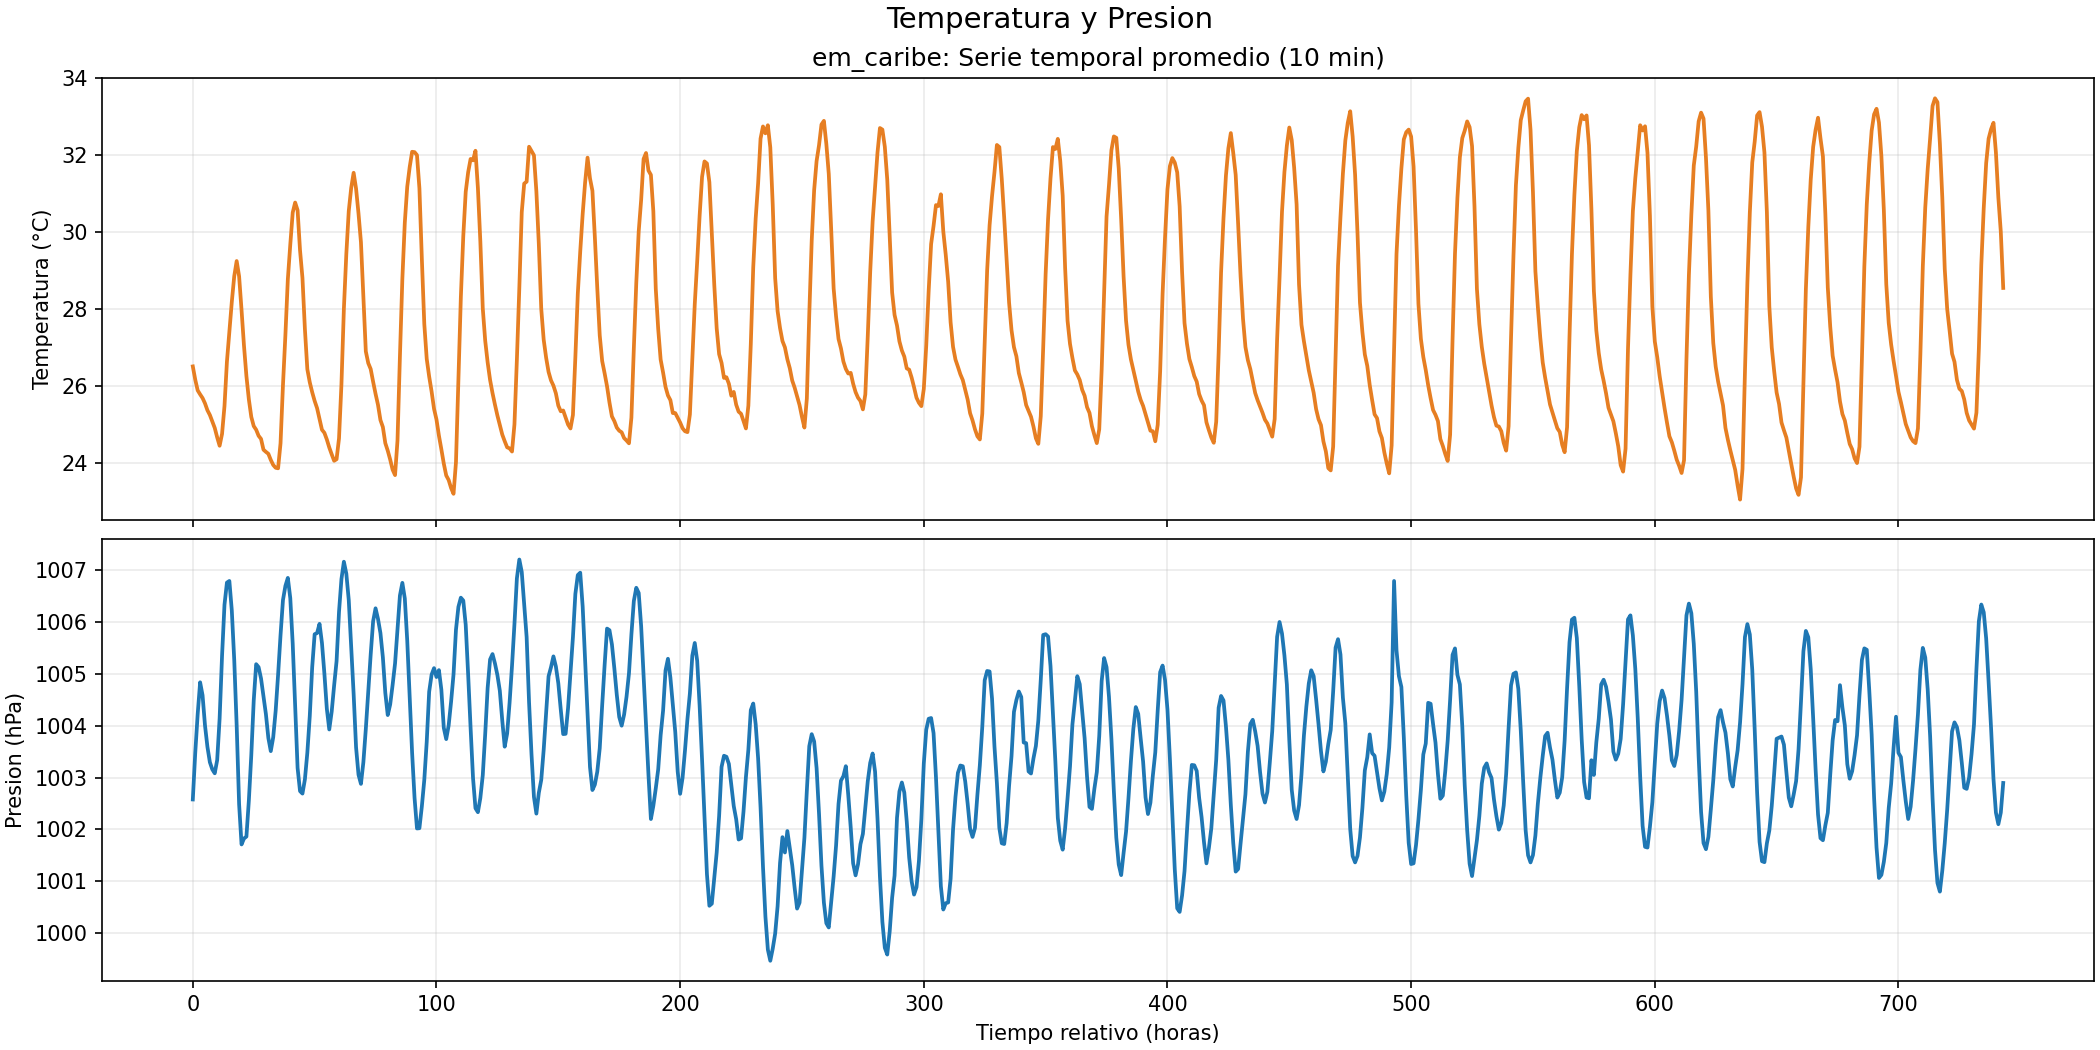
\includegraphics[width=0.80\textwidth]{Imagenes/descripcion_datos/em_caribe_temp_presion_time_series.png}
\caption{Serie temporal de temperatura y presion del conjunto Caribe para diciembre de 2025. Se evidencia variabilidad temporal apreciable en el periodo de entrenamiento.}
\label{fig:serie_temporal_datos_caribe}
\end{figure}

Como complemento de la caracterizacion temporal, la Figura~\ref{fig:serie_temporal_ux_uy_caribe} presenta la evolucion de las componentes del viento $u_x$ y $u_y$ en el periodo analizado. Esta evidencia permite contextualizar la variabilidad dinamica de las variables de salida principales del modelo.

\begin{figure}[H]
\centering
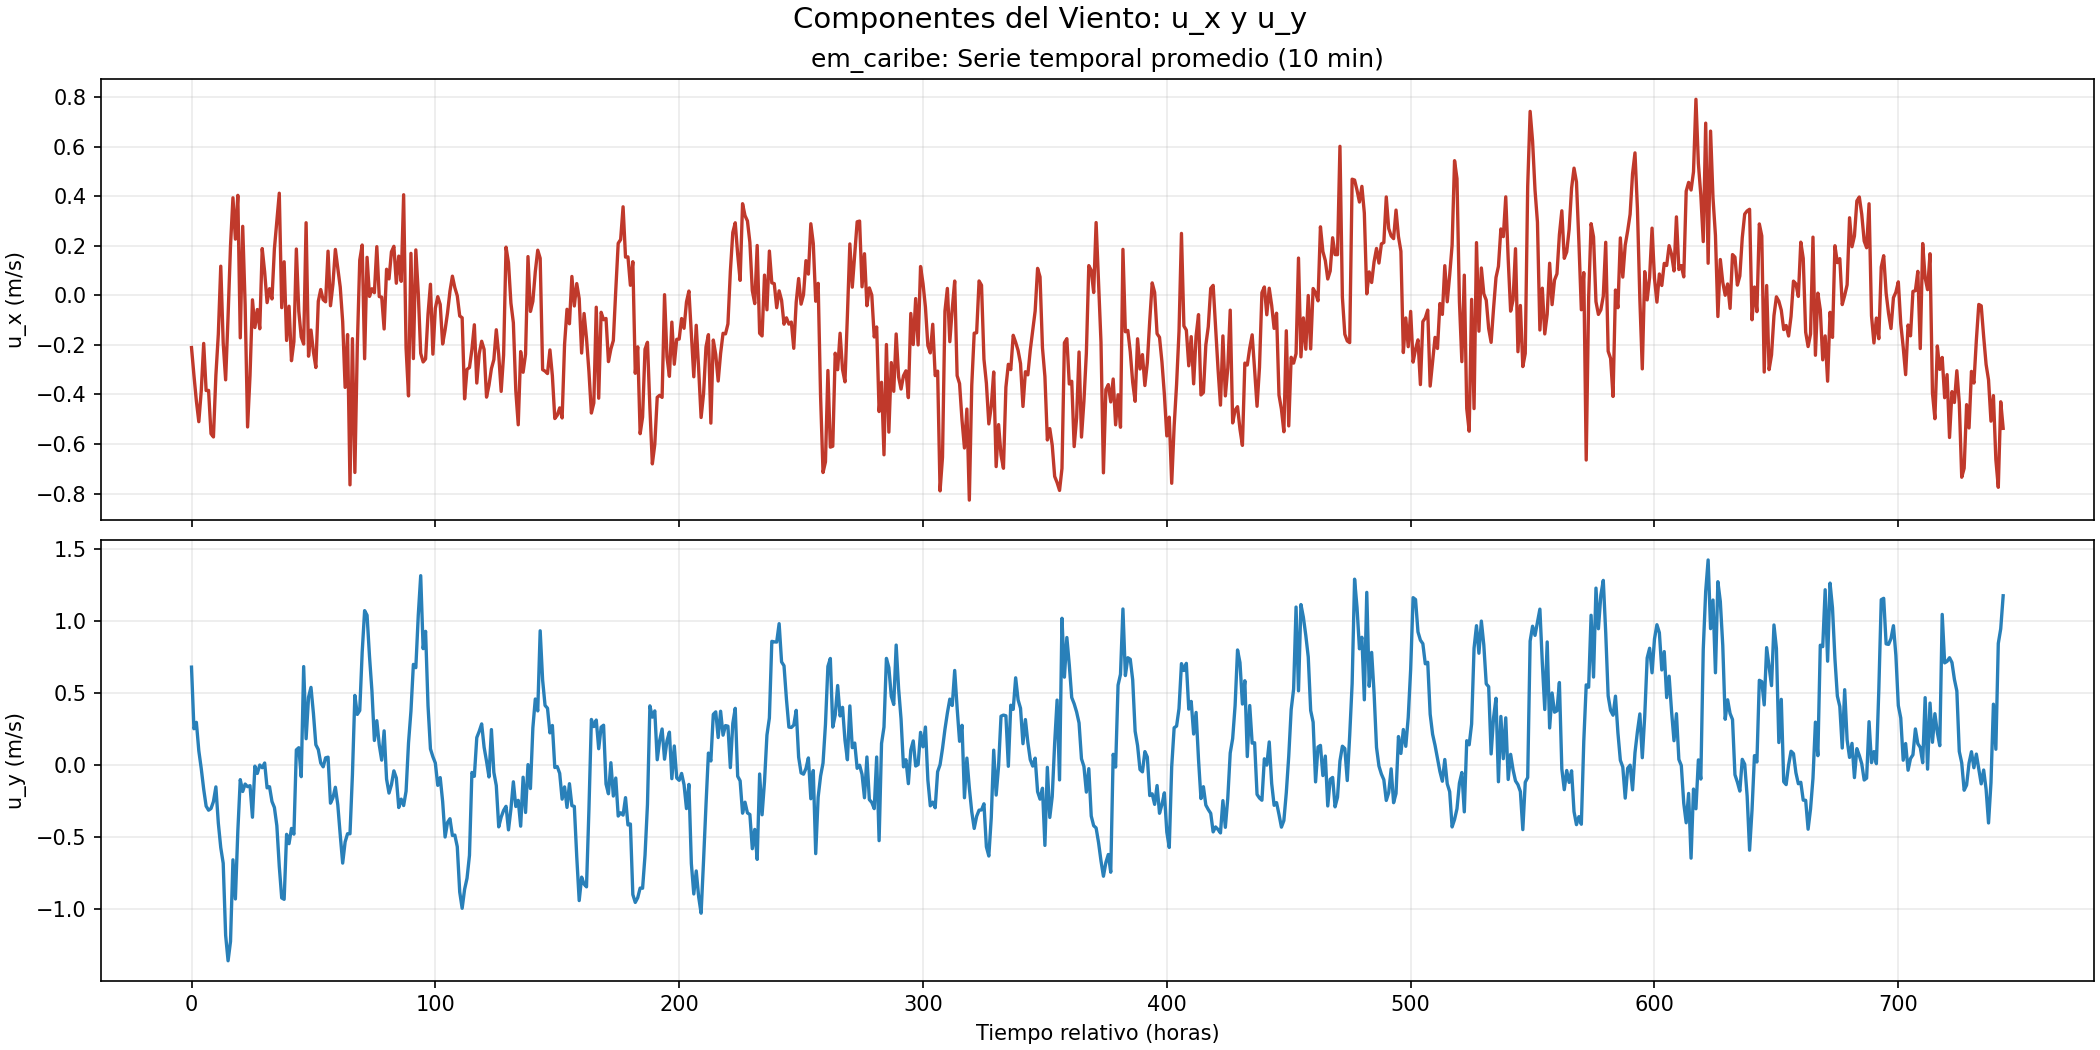
\includegraphics[width=0.90\textwidth]{Imagenes/descripcion_datos/em_caribe_ux_uy_time_series.png}
\caption{Serie temporal promedio de las componentes del viento $u_x$ y $u_y$ para el conjunto Caribe durante diciembre de 2025. La figura complementa la caracterizacion temporal de las variables meteorologicas empleadas en el estudio.}
\label{fig:serie_temporal_ux_uy_caribe}
\end{figure}

La Figura~\ref{fig:hist_temp_caribe} presenta la distribucion de temperatura del conjunto analizado. Este resumen descriptivo complementa la configuracion experimental al mostrar la concentracion de observaciones en un rango principal y la presencia de valores menos frecuentes en los extremos, condicion que es relevante para interpretar el comportamiento de la funcion de perdida durante el entrenamiento.

\begin{figure}[H]
\centering
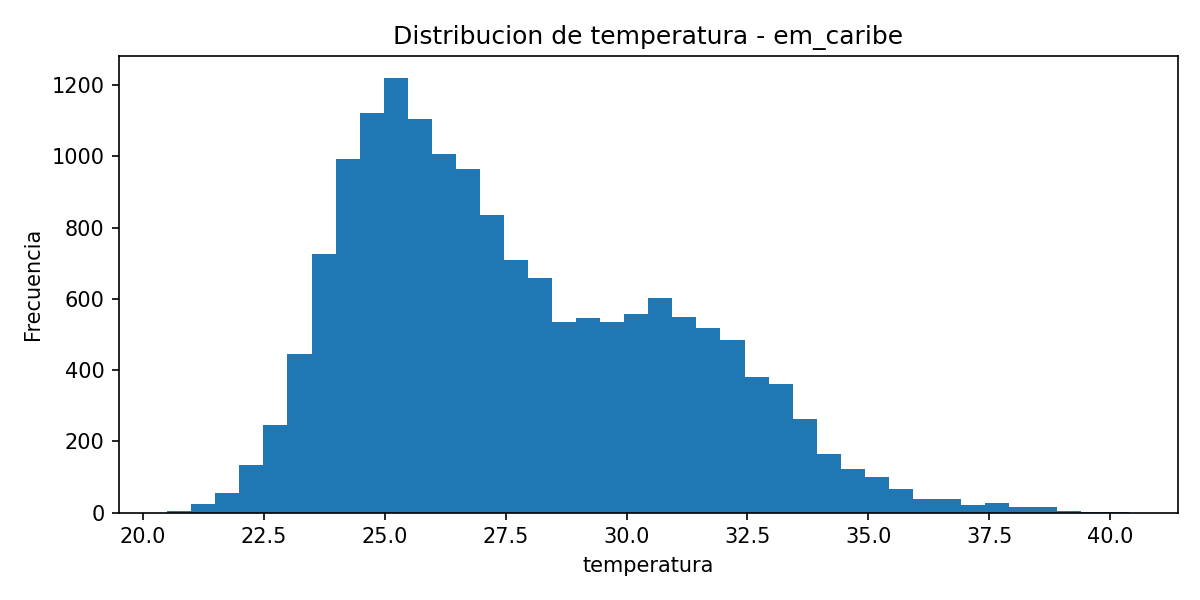
\includegraphics[width=0.80\textwidth]{Imagenes/descripcion_datos/em_caribe_temp_hist.png}
\caption{Histograma de temperatura del conjunto Caribe para diciembre de 2025. La figura se usa como apoyo descriptivo para contextualizar la distribucion de una variable de entrada clave del modelo.}
\label{fig:hist_temp_caribe}
\end{figure}

\section{Tabla maestra de experimentos evaluados}

La Tabla~\ref{tab:maestra_resultados} resume las corridas evaluadas de forma reproducible con métricas de la época 2.000. Cada fila corresponde a una configuración única de $(R, \lambda)$, con sus respectivos errores observacionales y residual físico.

\begin{table}[H]
\centering
\caption{Resultados consolidados de experimentos evaluados a época 2.000}
\label{tab:maestra_resultados}
\begin{tabular}{lcccccccc}
\hline
Modelo & $R$ & $\lambda$ & Reg./est. & Loss final & $\text{MSE}_{u_x}$ & $\text{MSE}_{u_y}$ & $\text{MSE}_{p}$ & $\mathcal{R}_{\text{NS}}$ \\
\hline
\texttt{todos\_R01\_L5} & 0,1 & 5 & $\sim744$ & 0,9261 & 0,4633 & 0,4347 & 1,3688 & \textbf{0,01273} \\
\texttt{300xest\_R01\_L5} & 0,1 & 5 & 300 & 1,1207 & 0,4689 & 0,4647 & 1,6220 & 0,03682 \\
\texttt{300xest\_R04\_L1} & 0,4 & 1 & 300 & 1,0575 & 0,5059 & 0,5085 & 1,5720 & 0,24141 \\
\texttt{300xest\_R01\_L1} & 0,1 & 1 & 300 & 1,1380 & 0,4806 & 0,4756 & 1,6477 & 0,20107 \\
\texttt{300xest\_R04\_L10} & 0,4 & 10 & 300 & 1,0859 & 0,5220 & 0,5224 & 1,6185 & 0,02242 \\
\texttt{300xest\_R01\_L10} & 0,1 & 10 & 300 & 1,1624 & 0,4919 & 0,4966 & 1,6906 & 0,02318 \\
\texttt{300xest\_R04\_L3} & 0,4 & 3 & 300 & 1,2357 & 0,6150 & 0,6274 & 1,8239 & 0,05974 \\
\texttt{300xest\_R01\_L3} & 0,1 & 3 & 300 & 1,6271 & 0,6921 & 0,6847 & 2,3727 & 0,11364 \\
\texttt{300xest\_R04\_L5} & 0,4 & 5 & 300 & 1,6203 & 0,7710 & 0,7817 & 2,4111 & 0,07074 \\
\hline
\end{tabular}
\end{table}

\noindent\textit{Nota:} La corrida extendida con restriccion suave de rango (\texttt{todosreg\_R01\_L5\_rangeL05}) se reporta de forma explicita en la Subseccion de efecto de la restriccion suave de rango, dentro de este mismo capitulo.

El mejor desempeño global se obtuvo con la corrida \texttt{todos\_R01\_L5}, que utiliza la totalidad de los datos disponibles (aproximadamente 744 registros por estación) con resolución de malla R = 0,1° y peso físico $\lambda = 5$. Esta configuración alcanza simultáneamente el menor error observacional promedio (0,7556) y el menor residual de Navier-Stokes (0,01273) entre todos los experimentos evaluados.

\section{Ranking por error observacional promedio}

Se utilizo el criterio:

\[
\bar{MSE}_{obs}=\frac{\text{MSE}_{u_x}+\text{MSE}_{u_y}+\text{MSE}_{p}}{3}
\]

La Tabla~\ref{tab:ranking_obs} presenta el ranking consolidado.

\begin{table}[H]
\centering
\caption{Ranking por error observacional promedio}
\label{tab:ranking_obs}
\begin{tabular}{clcc}
\hline
Pos. & Modelo & $\bar{MSE}_{obs}$ & Residual NS \\
\hline
1 & \texttt{todos\_R01\_L5} & 0,75559 & 0,01273 \\
2 & \texttt{300xest\_R01\_L5} & 0,85185 & 0,03682 \\
3 & \texttt{300xest\_R04\_L1} & 0,86216 & 0,24141 \\
4 & \texttt{300xest\_R01\_L1} & 0,86796 & 0,20107 \\
5 & \texttt{300xest\_R04\_L10} & 0,88765 & 0,02242 \\
6 & \texttt{300xest\_R01\_L10} & 0,89305 & 0,02318 \\
7 & \texttt{300xest\_R04\_L3} & 1,02208 & 0,05974 \\
8 & \texttt{300xest\_R01\_L3} & 1,24982 & 0,11364 \\
9 & \texttt{300xest\_R04\_L5} & 1,32126 & 0,07074 \\
\hline
\end{tabular}
\end{table}

\section{Analisis por factores}

\subsection{Efecto de \texorpdfstring{$\lambda$ en $R=0{,}1^{\circ}$}{lambda en R=0,1 grados} (resolución fina)}

En el bloque de malla fina con 91.200 puntos de colocación, el efecto del peso físico $\lambda$ presenta un comportamiento no monótono:

\begin{table}[H]
\centering
\begin{tabular}{cccc}
\hline
$\lambda$ & $\overline{\text{MSE}}_{\text{obs}}$ & $\mathcal{R}_{\text{NS}}$ & Caracterización \\
\hline
1 & 0,86796 & 0,20107 & Balance moderado, residual alto \\
3 & 1,24982 & 0,11364 & Peor resultado del bloque \\
5 & \textbf{0,85185} & \textbf{0,03682} & \textbf{Mejor equilibrio obs-físico} \\
10 & 0,89305 & 0,02318 & Residual mínimo, velocidades degradadas \\
\hline
\end{tabular}
\caption{Efecto de $\lambda$ en $R=0{,}1^{\circ}$: evolución de error observacional y residual físico.}
\label{tab:lambda_r01}
\end{table}

El valor $\lambda = 5$ emerge como óptimo en este bloque, equilibrando ajuste observacional y satisfacción de las restricciones físicas. Notablemente, $\lambda = 3$ produce degradación sistemática en ambos criterios.

\subsection{Efecto de \texorpdfstring{$\lambda$ en $R=0{,}4^{\circ}$}{lambda en R=0,4 grados} (resolución gruesa)}

En el bloque de malla gruesa \((R=0{,}4^{\circ})\), con 13.200 puntos de colocación, se observa un compromiso claro entre desempeño observacional y cumplimiento físico: $\lambda=1$ logra el mejor ajuste observacional $\left(\overline{\text{MSE}}_{\text{obs}}=0{,}86216\right)$ pero con residual elevado $\left(\mathcal{R}_{\text{NS}}=0{,}24141\right)$, mientras que $\lambda=10$ obtiene el residual mínimo del bloque $\left(\mathcal{R}_{\text{NS}}=0{,}02242\right)$ con una pérdida moderada en el ajuste observacional $\left(\overline{\text{MSE}}_{\text{obs}}=0{,}88765\right)$; por su parte, $\lambda=3$ presenta comportamiento intermedio $\left(\overline{\text{MSE}}_{\text{obs}}=1{,}02208,\ \mathcal{R}_{\text{NS}}=0{,}05974\right)$ y $\lambda=5$ concentra el peor desempeño observacional del bloque $\left(\overline{\text{MSE}}_{\text{obs}}=1{,}32126,\ \mathcal{R}_{\text{NS}}=0{,}07074\right)$, lo que confirma que en esta resolución no existe un valor único dominante para ambos criterios y que el incremento de $\lambda$ favorece la restricción física en detrimento parcial del ajuste a observaciones.

\subsection{Patrón crítico: insuficiencia de \texorpdfstring{$\lambda = 3$}{lambda = 3}}

Un hallazgo metodológico relevante es que $\lambda = 3$ presenta desempeño consistentemente desfavorable en ambas resoluciones de malla. La Tabla~\ref{tab:lambda_r01} y los resultados descritos en la sección anterior muestran que este valor específico genera una tensión desequilibrada entre objetivos observacional y físico, resultando en errores superiores a las alternativas adyacentes ($\lambda = 1$ y $\lambda = 5$).

\subsection{Efecto de la resolucion de malla}

Comparando pares equivalentes con $\lambda$ fijo pero $R$ diferente:

\begin{table}[H]
\centering
\begin{tabular}{ccccc}
\hline
$\lambda$ & $\overline{\text{MSE}}_{\text{obs}}$ R=0,1 & $\overline{\text{MSE}}_{\text{obs}}$ R=0,4 & Diferencia & Mejor R \\
\hline
1 & 0,86796 & 0,86216 & -0,0058 (marginal) & 0,4 \\
3 & 1,24982 & 1,02208 & -0,2277 (marcado) & 0,4 \\
5 & 0,85185 & 1,32126 & +0,4694 (marcado) & \textbf{0,1} \\
10 & 0,89305 & 0,88765 & -0,0054 (marginal) & 0,4 \\
\hline
\end{tabular}
\caption{Comparación de resoluciones: R = 0,4° domina en $\lambda \in \{1, 3, 10\}$, pero R = 0,1° es superior en $\lambda = 5$.}
\label{tab:efecto_resolucion}
\end{table}

Este resultado sugiere que la densidad de puntos de colocación modula la efectividad del peso físico. Una malla más fina (R = 0,1°) requiere un $\lambda$ mayor para controlar el comportamiento sobre los puntos adicionales de colocación; con $\lambda$ bajo, los puntos extras quedan infrautilizados.

\subsection{Efecto del volumen de datos}

La corrida final utilizó la totalidad de los registros disponibles, manteniendo la configuración óptima identificada en el barrido (R = 0,1°, $\lambda = 5$). Con la misma arquitectura y configuración de entrenamiento, el incremento de datos produjo mejoras sustanciales:

\begin{table}[H]
\centering
\begin{tabular}{lccc}
\hline
Configuración & Registros totales & $\overline{\text{MSE}}_{\text{obs}}$ & $\mathcal{R}_{\text{NS}}$ \\
\hline
\texttt{300xest\_R01\_L5} & 5.400 & 0,85185 & 0,03682 \\
\texttt{todos\_R01\_L5} & 13.392 & 0,75559 & 0,01273 \\
\hline
Mejora (reducción \%) & 2,48× más & -11,3\% & -65,4\% \\
\hline
\end{tabular}
\caption{Impacto del volumen de datos: con 744 registros/estación (~13.392 en total) frente a 300 registros/estación (5.400 total), manteniendo R = 0,1° y $\lambda = 5$.}
\label{tab:efecto_volumen}
\end{table}

El incremento de 2,48× en el volumen de datos resultó en reducción del 11,3\% del error observacional promedio y del 65,4\% del residual de Navier-Stokes. Este resultado indica que el modelo PINN aún operaba en régimen de datos limitados durante el barrido, y que la cobertura temporal ampliada es una palanca efectiva de mejora sin cambios arquitecturales.

\subsection{Efecto de la restriccion suave de rango}

Como extension metodologica del estudio, se evaluo una corrida adicional con restriccion suave de rango sobre la configuracion de referencia $R=0{,}1^\circ$, $\lambda=5$, denominada \texttt{todosreg\_R01\_L5\_rangeL05}. Esta variante incorporo cuantiles robustos, penalizacion softplus y una rampa lineal para el peso $\lambda_R$ dentro de la funcion de perdida extendida.

La Tabla~\ref{tab:range_loss_comp} compara tres escenarios con arquitectura comun y la misma pareja $(R,\lambda)=(0{,}1,5)$, diferenciados por volumen de datos y por la activacion del mecanismo de rango.

\begin{table}[H]
\centering
\begin{tabular}{lccc}
\hline
Experimento & Registros totales & Mecanismo de rango & Loss final \\
\hline
\texttt{300xest\_R01\_L5} & 5.400 & No & 1,117 \\
\texttt{todos\_R01\_L5} & 13.392 & No & 0,926 \\
\texttt{todosreg\_R01\_L5\_rangeL05} & 13.392 & Si & \textbf{0,638} \\
\hline
\end{tabular}
\caption{Comparacion de perdida final a epoca 2.000 en escenarios de referencia con y sin restriccion suave de rango.}
\label{tab:range_loss_comp}
\end{table}

Para verificar si la reduccion de la perdida total se traduce en un beneficio genuino sobre el ajuste observacional y no solamente en la satisfaccion del termino de penalizacion de rango, se evaluaron las metricas desagregadas del modelo de referencia frente al modelo con restriccion de rango. La Tabla~\ref{tab:range_metricas_comp} presenta esta comparacion.

\begin{table}[H]
\centering
\caption{Metricas comparativas entre el modelo base y el modelo con restriccion de rango}
\label{tab:range_metricas_comp}
\begin{tabular}{lccc}
\hline
Metrica & \texttt{todos\_R01\_L5} & \texttt{todosreg\_R01\_L5\_rangeL05} & Variacion \\
\hline
$\text{MSE}_{u_x}$ & 0,4633 & 0,3799 & $-18{,}0\%$ \\
$\text{MSE}_{u_y}$ & 0,4347 & 0,3775 & $-13{,}2\%$ \\
$\text{MSE}_{p}$ & 1,3688 & 0,9875 & $-27{,}9\%$ \\
$\mathcal{R}_{\text{NS}}$ & 0,01273 & 0,01534 & $+20{,}5\%$ \\
Loss total & 0,926 & \textbf{0,638} & $-31{,}1\%$ \\
\hline
\end{tabular}
\end{table}

\noindent\textit{Nota: variables en unidades normalizadas. MSE calculado sobre los puntos de las estaciones; $\mathcal{R}_{\text{NS}}$ sobre los puntos de colocacion.}

Los resultados indican que la incorporacion de la restriccion de rango produce una mejora real en el ajuste observacional: el MSE disminuye entre 13\,\% y 28\,\% para las tres variables de salida con respecto al modelo base. Esta mejora no es un artefacto de la funcion de perdida: el termino de penalizacion de rango actua sobre los puntos de la malla, no sobre los puntos de las estaciones donde se calcula el MSE. La reduccion del MSE observacional refleja por tanto una regularizacion implicita del campo de prediccion: al forzar que las predicciones en zonas no observadas permanezcan dentro de rangos plausibles, el modelo evita soluciones patologicas que propaguen errores hacia las regiones con estaciones.

No obstante, la restriccion de rango presenta dos efectos secundarios que deben considerarse. Primero, el residual de Navier-Stokes aumenta levemente ($\mathcal{R}_{\text{NS}}$: 0,01273 $\to$ 0,01534, $+20{,}5$\,\%), lo que indica que la penalizacion de rango compite parcialmente con la restriccion fisica durante el entrenamiento. Segundo, el porcentaje de predicciones fuera de rango en la malla completa permanece elevado para las componentes de velocidad ($\text{FOR}_{u} = 64{,}35$\,\%, $\text{FOR}_{v} = 48{,}09$\,\%), lo que sugiere que la red no alcanza la cobertura completa del rango en las 2.000 epocas evaluadas. La presion, en cambio, logra compliance casi total ($\text{FOR}_{p} = 0{,}28$\,\%). Este comportamiento asimetrico puede deberse a la mayor variabilidad espacial de las componentes de velocidad o a que el valor $\lambda_{R,\max} = 0{,}50$ no es suficiente para reducir FOR en velocidades dentro del horizonte de entrenamiento disponible.

En conjunto, la restriccion de rango mejora el ajuste observacional y reduce la perdida total, pero la elevada FOR en velocidades indica que el experimento no ha convergido completamente hacia el cumplimiento de la restriccion. La optimizacion de $\lambda_{R,\max}$ y del numero de epocas queda como linea de trabajo futuro.

\begin{figure}[H]
\centering
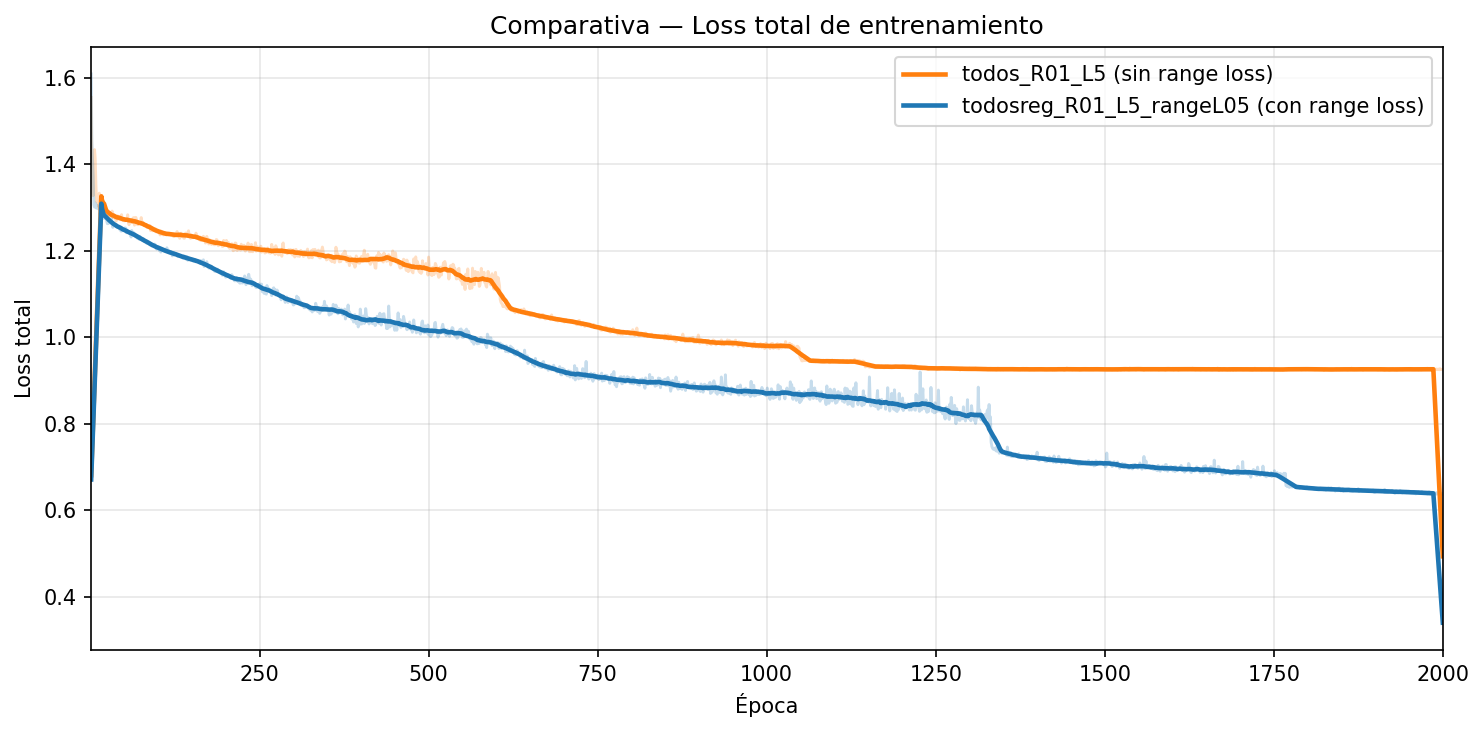
\includegraphics[width=0.92\textwidth]{Imagenes/rango/01_loss_total_comparativa.png}
\caption{Comparacion de la perdida total durante el entrenamiento para escenarios de referencia con y sin restriccion suave de rango.}
\label{fig:range_loss_total_comp}
\end{figure}

Como resultado final del entrenamiento con restriccion suave de rango, las Figuras~\ref{fig:range_campo_u}, \ref{fig:range_campo_v} y \ref{fig:range_campo_p} presentan los campos predichos para las componentes de velocidad y la presion en la corrida \texttt{todosreg\_R01\_L5\_rangeL05}.

\begin{figure}[H]
\centering
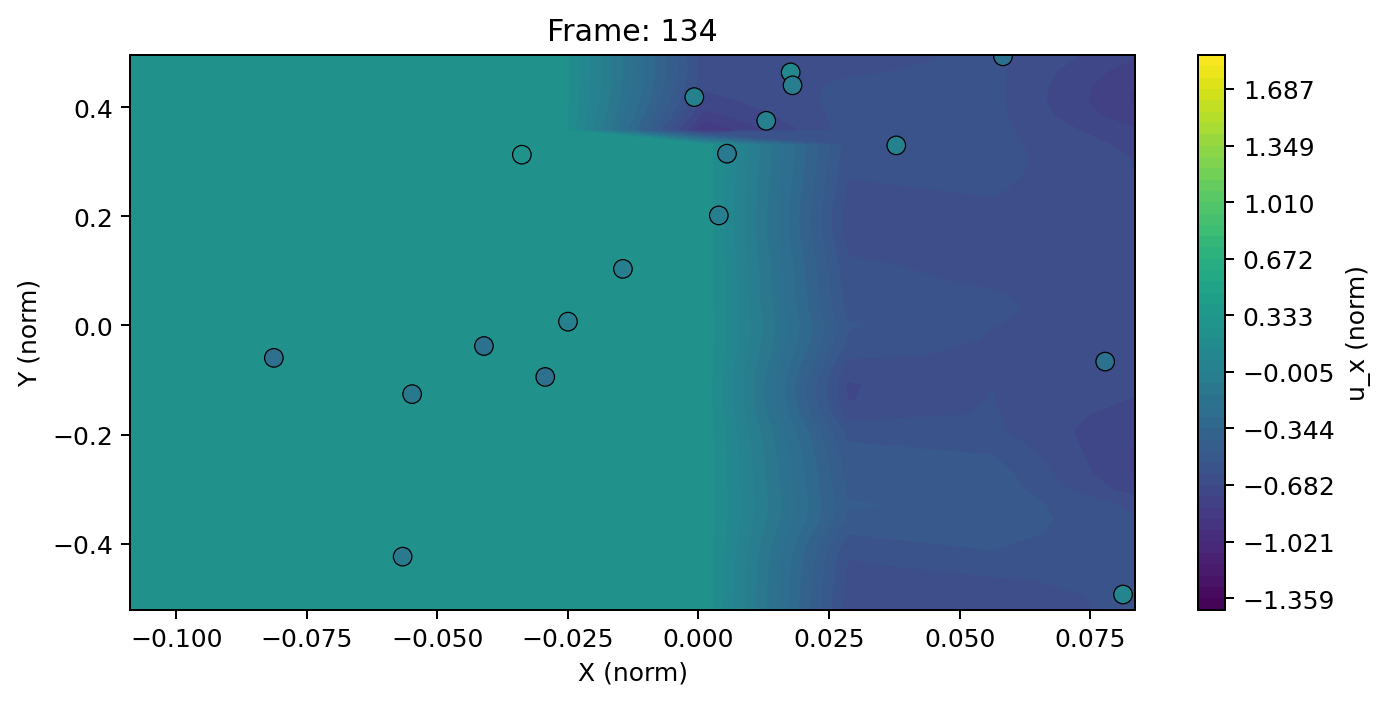
\includegraphics[width=0.92\textwidth]{Imagenes/rango/pinn_caribe_excl4_todosreg_r01_l5_rangel05_epoca_2000_frame_min_loss_general_u_t134.png}
\caption{Campo predicho final de $u$ para la corrida \texttt{todosreg\_R01\_L5\_rangeL05}.}
\label{fig:range_campo_u}
\end{figure}

\begin{figure}[H]
\centering
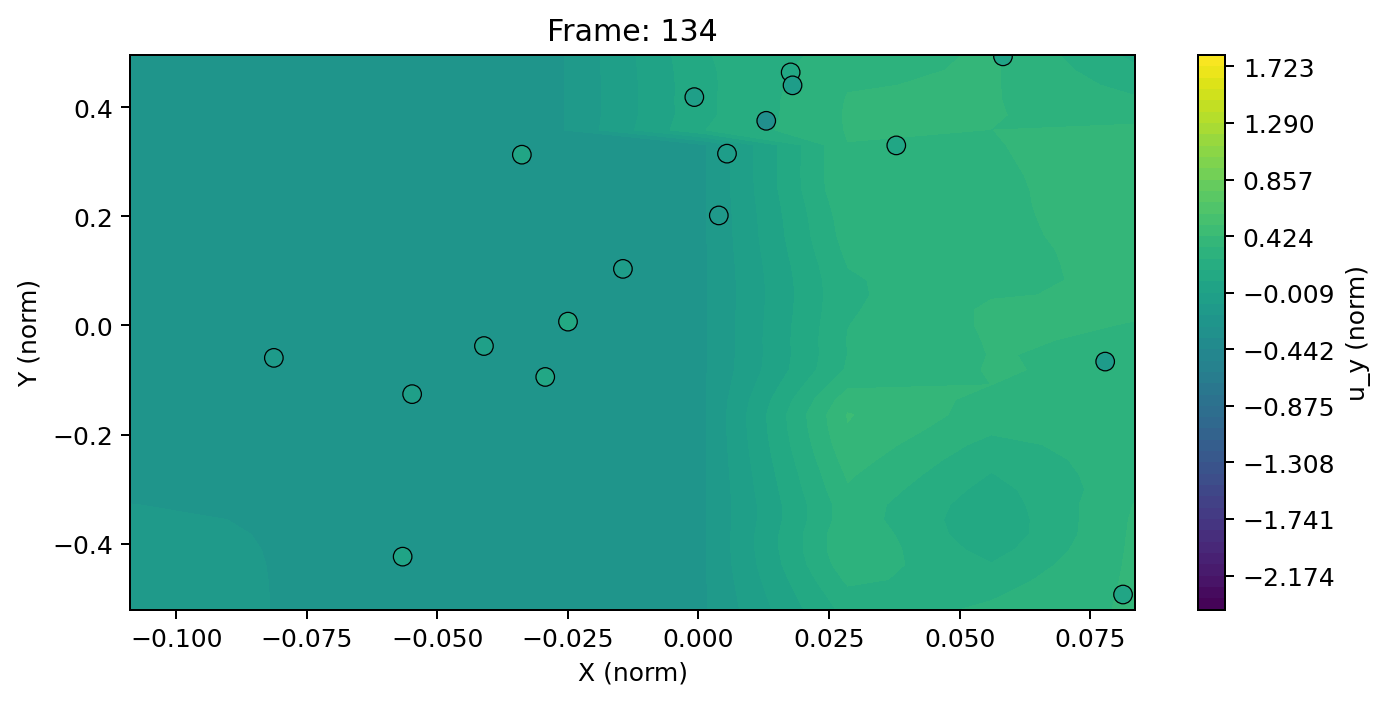
\includegraphics[width=0.92\textwidth]{Imagenes/rango/pinn_caribe_excl4_todosreg_r01_l5_rangel05_epoca_2000_frame_min_loss_general_v_t134.png}
\caption{Campo predicho final de $v$ para la corrida \texttt{todosreg\_R01\_L5\_rangeL05}.}
\label{fig:range_campo_v}
\end{figure}

\begin{figure}[H]
\centering
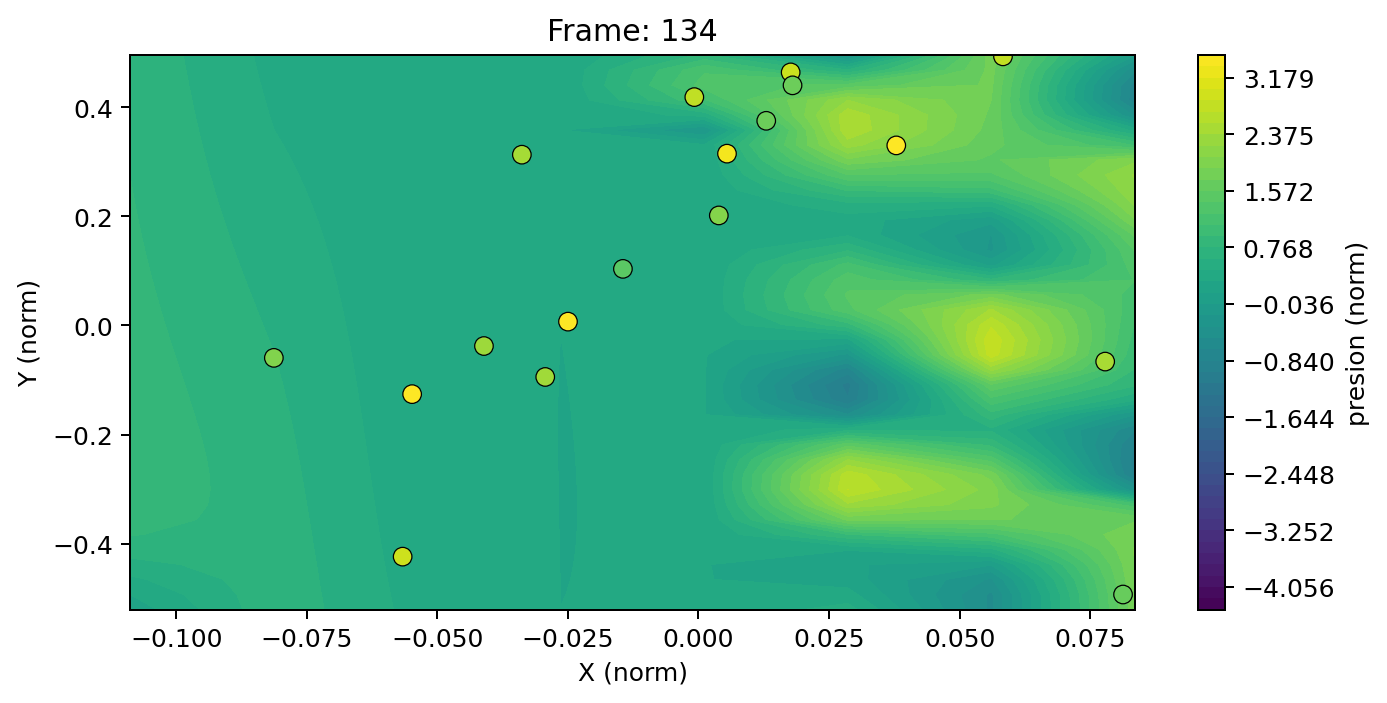
\includegraphics[width=0.92\textwidth]{Imagenes/rango/pinn_caribe_excl4_todosreg_r01_l5_rangel05_epoca_2000_frame_min_loss_general_p_t134.png}
\caption{Campo predicho final de $p$ para la corrida \texttt{todosreg\_R01\_L5\_rangeL05}.}
\label{fig:range_campo_p}
\end{figure}

\begin{figure}[H]
\centering
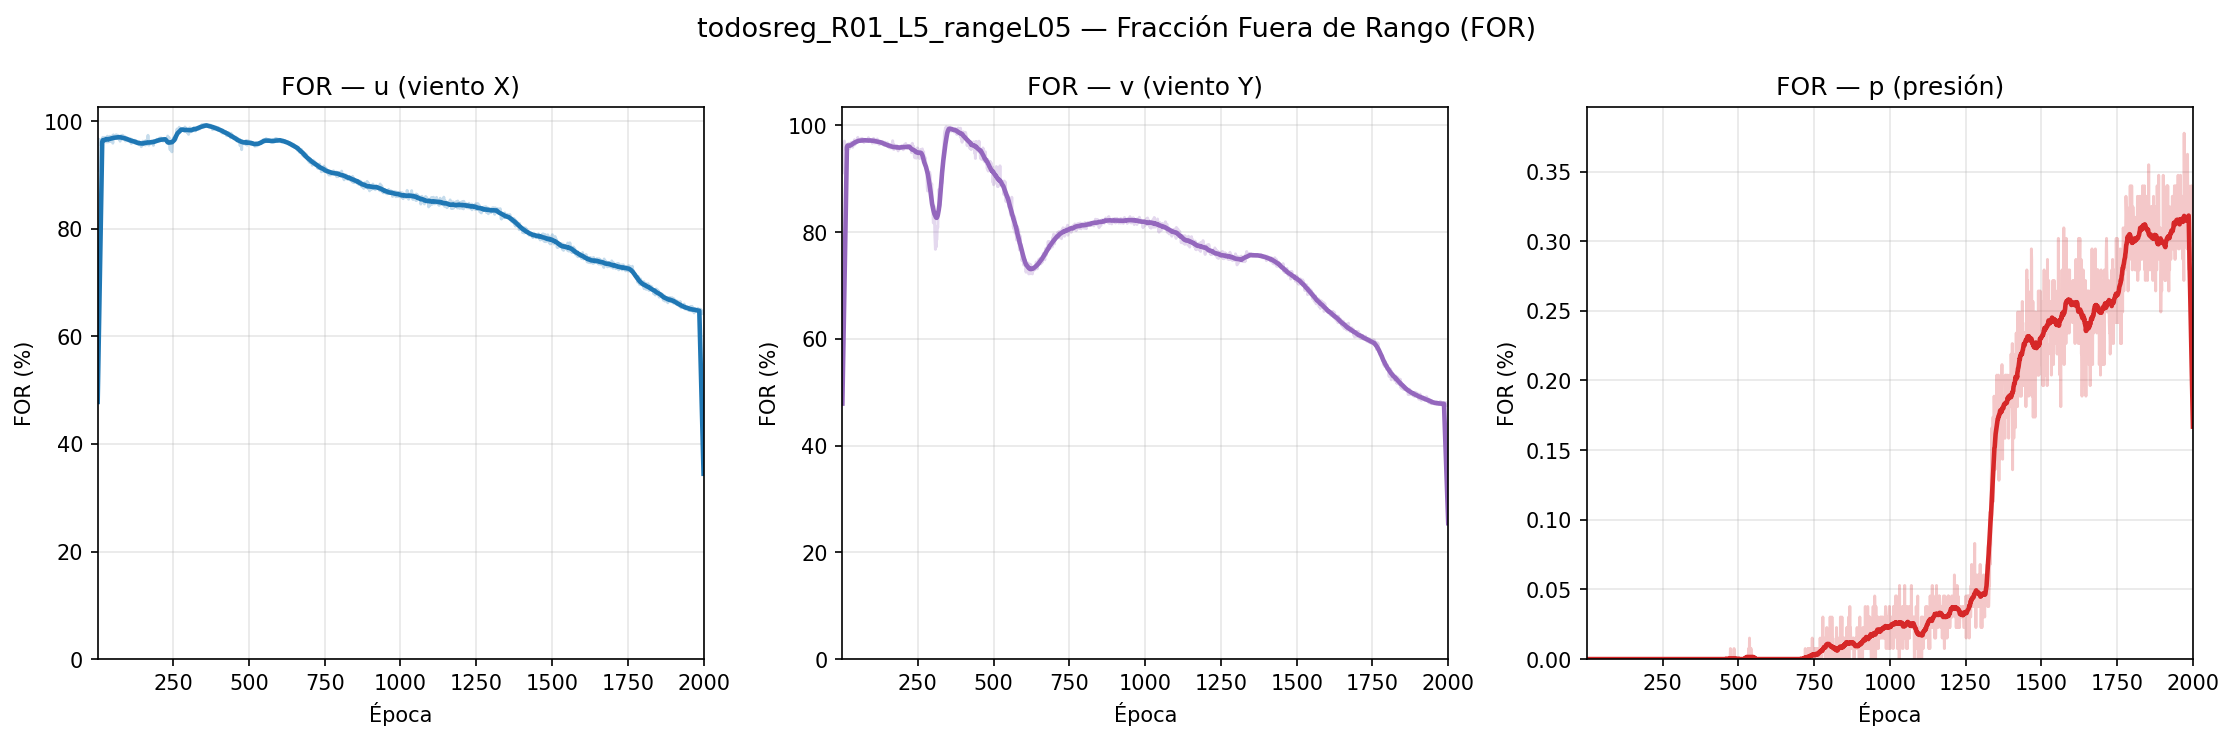
\includegraphics[width=0.92\textwidth]{Imagenes/rango/05_for_metricas.png}
\caption{Evolucion de la metrica FOR para las variables de salida en la corrida con restriccion suave de rango.}
\label{fig:range_for_metricas}
\end{figure}

\section{Validación fuera de muestra: generalización temporal}

Para evaluar la capacidad de generalización del modelo a condiciones temporales no vistas
durante el entrenamiento, se realizó una partición temporal del conjunto de datos:
los días 1 a 20 de diciembre de 2025 (8.574 registros) se utilizaron para el entrenamiento,
y los días 21 a 31 (4.818 registros) constituyeron el conjunto de prueba independiente.
Se entrenó el modelo con la configuración de referencia ($R = 0{,}1^{\circ}$, $\lambda = 5{,}0$,
2.000 épocas, todas las estaciones activas) y se evaluaron las métricas $\text{MSE}_{\text{obs}}$
y $\mathcal{R}_{\text{NS}}$ sobre el conjunto de prueba una vez completado el entrenamiento.
La Tabla~\ref{tab:validacion_prueba} compara las métricas obtenidas en entrenamiento y en prueba.
Los valores de referencia del entrenamiento corresponden al modelo \texttt{todos\_R01\_L5}
(entrenado con los 31 días completos) y se incluyen como referencia de escala para las variables
en unidades normalizadas.

\begin{table}[H]
\centering
\caption{Comparación de métricas entre el conjunto de entrenamiento (días 1–20) y el conjunto de prueba (días 21–31) para el modelo \texttt{PINN\_caribe\_excl4\_todos\_R01\_L5\_train20d}}
\label{tab:validacion_prueba}
\begin{tabular}{lccc}
\hline
Métrica & Entrenamiento (días 1–20) & Prueba (días 21–31) & Diferencia \\
\hline
$\text{MSE}_{u_x}$ & 0{,}4633 & \textbf{0{,}4422} & $-4{,}5$\,\% \\
$\text{MSE}_{u_y}$ & 0{,}4347 & \textbf{0{,}4248} & $-2{,}3$\,\% \\
$\text{MSE}_{p}$   & 1{,}3688 & \textbf{3{,}9116} & $+185{,}8$\,\% \\
$\mathcal{R}_{\text{NS}}$ & 0{,}01273 & \textbf{0{,}03640} & $+186{,}0$\,\% \\
\hline
\end{tabular}
\end{table}

\noindent\textit{Nota: variables en unidades normalizadas. MSE calculado sobre los puntos de las
estaciones; $\mathcal{R}_{\text{NS}}$ sobre los puntos de colocación. Valores de referencia de entrenamiento tomados del modelo
\texttt{todos\_R01\_L5} (31 días completos).}

Los resultados evidencian un comportamiento diferenciado según la variable de salida.
Las componentes de velocidad del viento ($u_x$, $u_y$) muestran métricas de prueba
prácticamente idénticas a las de entrenamiento (diferencias de $-4{,}5$\,\% y $-2{,}3$\,\%
respectivamente), lo que sugiere que la restricción física de Navier-Stokes actúa como
regularizador efectivo para el campo de velocidades y permite una generalización temporal
satisfactoria a los 11 días no vistos durante el entrenamiento.

Sin embargo, el $\text{MSE}$ de presión aumenta de forma significativa en el conjunto de
prueba ($1{,}3688 \to 3{,}9116$, un incremento del $185{,}8$\,\%), indicando sobreajuste en la
variable de presión. Este comportamiento asimétrico es coherente con la naturaleza de los datos:
la presión atmosférica exhibe mayor variabilidad temporal y menor densidad observacional que las
componentes de velocidad, lo que reduce la capacidad del modelo para extrapolar su campo fuera
del período de entrenamiento. El residual de Navier-Stokes también aumenta en prueba
($0{,}01273 \to 0{,}03640$, $+186{,}0$\,\%), confirmando que las restricciones físicas aprendidas
sobre los primeros 20 días no se transfieren plenamente al período de prueba.

En conjunto, estos resultados sugieren que la PINN desarrollada tiene capacidad de
generalización temporal para el campo de viento, pero no para el campo de presión en el período
evaluado. Las predicciones de viento sobre días no vistos pueden considerarse razonablemente
confiables dentro del dominio y período estudiados, mientras que las predicciones de presión
deben interpretarse con cautela fuera del período de entrenamiento. Como líneas de mejora se
proponen: (1)~incorporar datos de presión de mayor resolución temporal, (2)~aumentar el peso
relativo de la pérdida física sobre la presión ($\lambda_p > \lambda_{\text{viento}}$),
o (3)~ampliar el período de entrenamiento a meses adicionales disponibles en el portal de
Datos Abiertos Colombia.

\section{Evidencia visual de configuraciones de referencia}

Las Figuras~\ref{fig:error_r01_l5} y~\ref{fig:mse_r01_l5} presentan el comportamiento temporal del error para \texttt{R01\_L5} (mejor corrida del bloque de 300 registros por estacion en $R=0{,}1^\circ$).

\begin{figure}[H]
\centering
\begin{subfigure}[b]{0.85\textwidth}
  \centering
  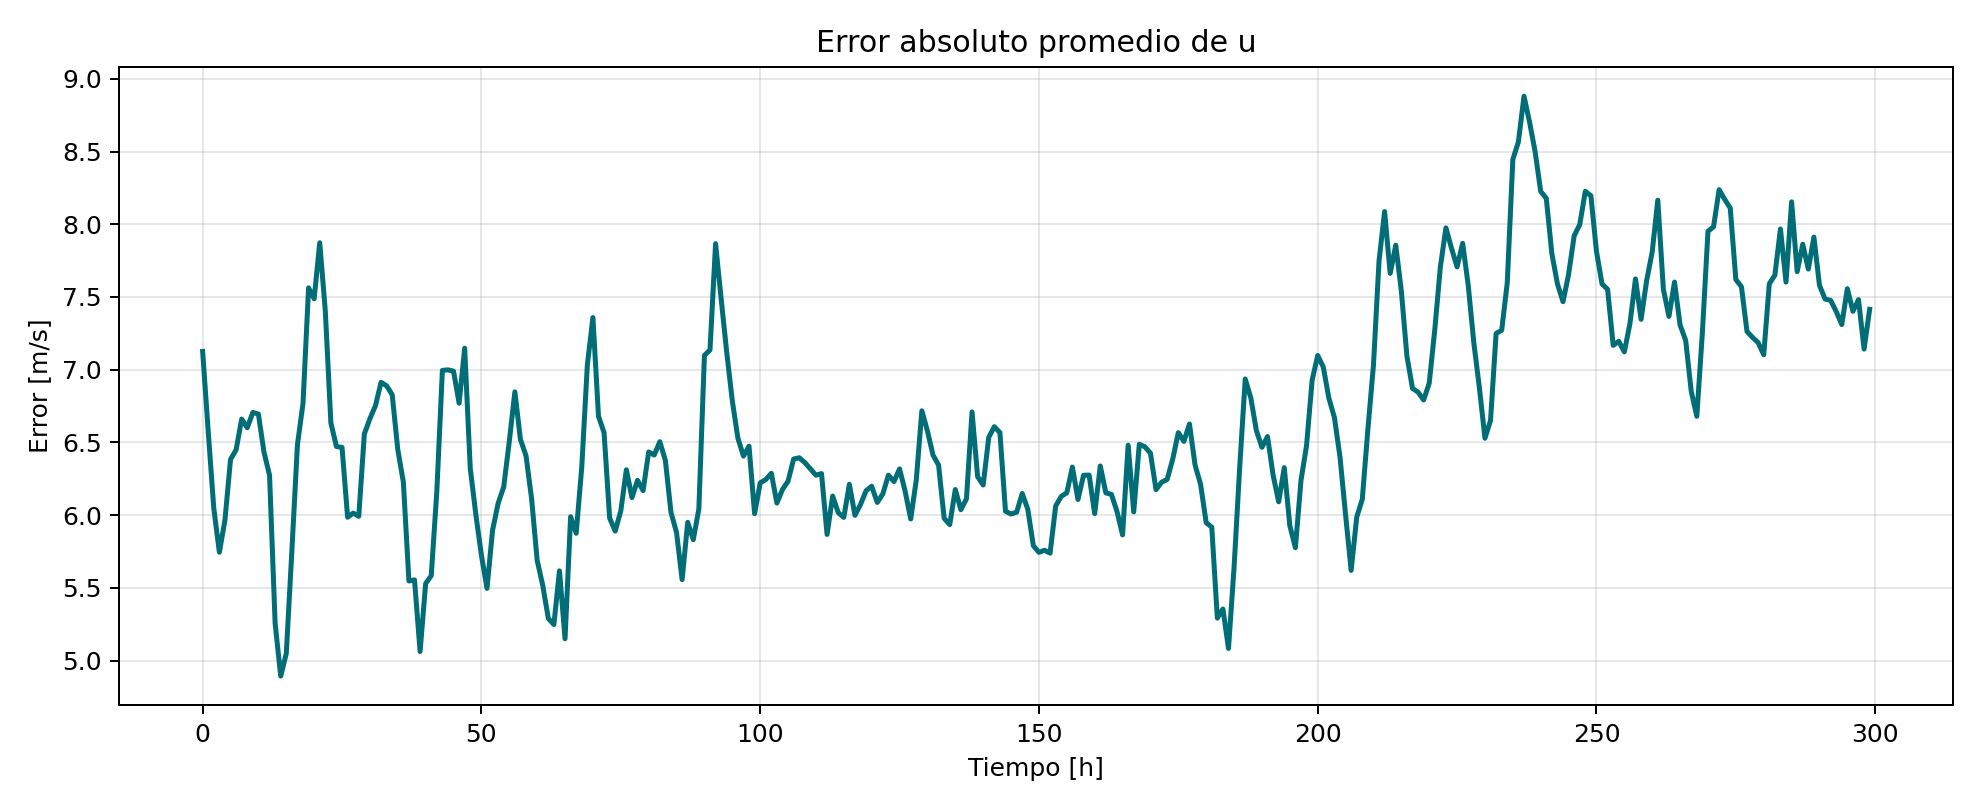
\includegraphics[width=\textwidth]{Imagenes/iter_R01/PINN_caribe_excl4_300xest_R01_L5/pinn_caribe_excl4_300xest_r01_l5_epoca_2000_error_promedio_u_tiempo.png}
  \caption{Error absoluto promedio de la componente $u$ (Este--Oeste) en m/s.}
\end{subfigure}
\par\medskip
\begin{subfigure}[b]{0.85\textwidth}
  \centering
  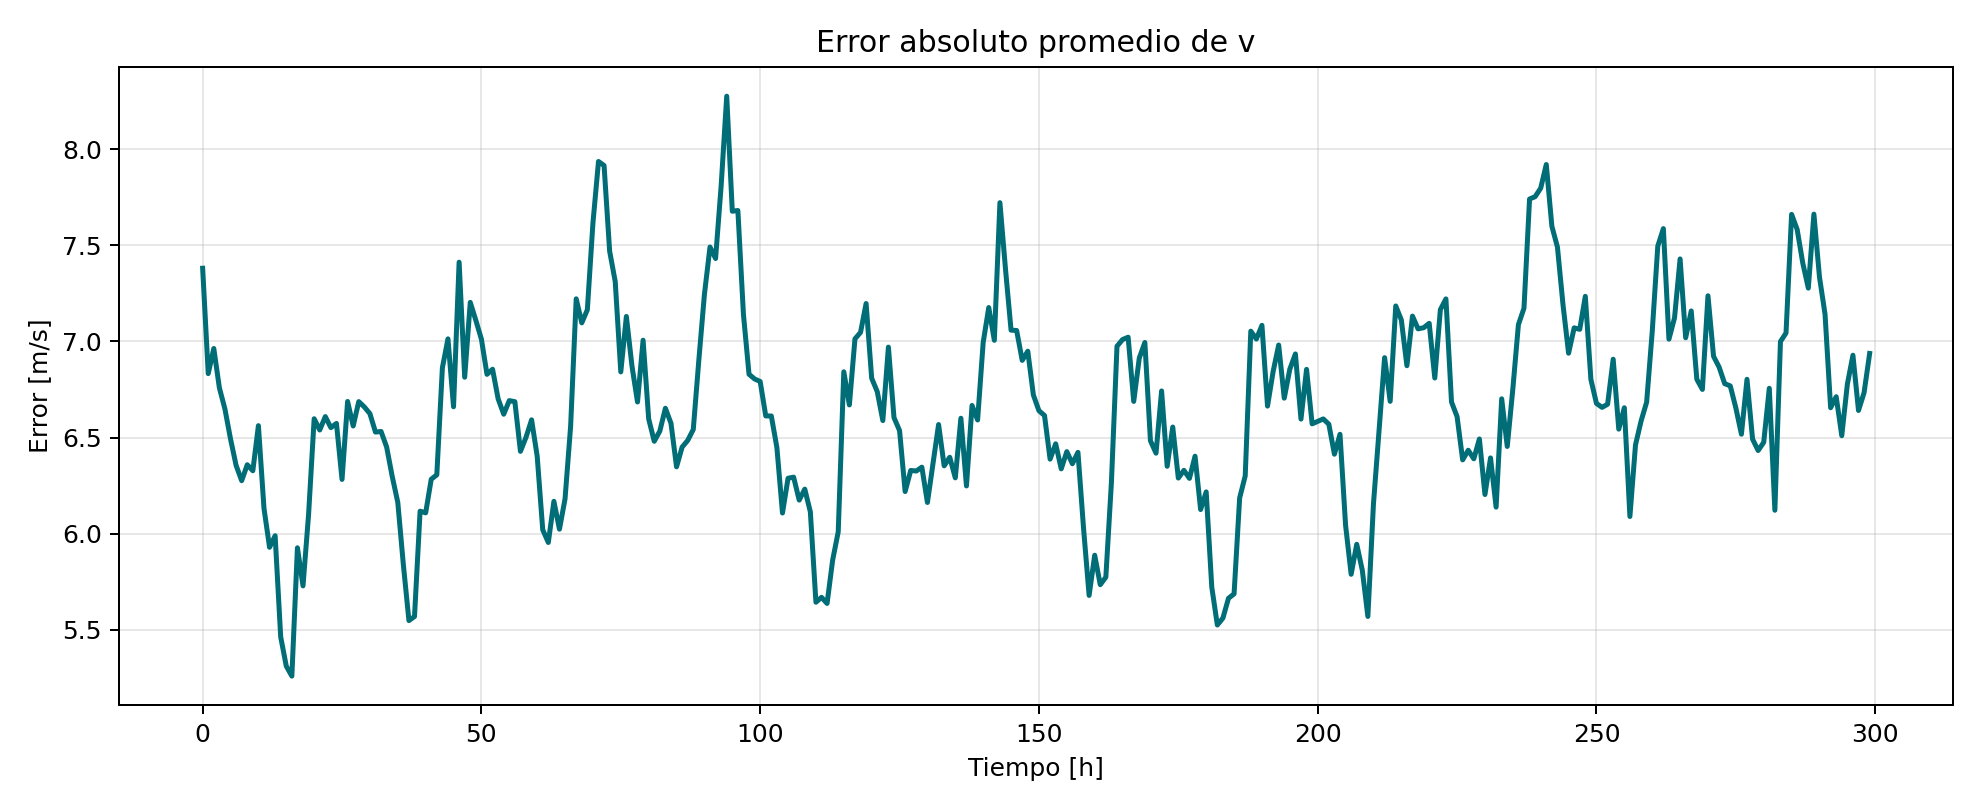
\includegraphics[width=\textwidth]{Imagenes/iter_R01/PINN_caribe_excl4_300xest_R01_L5/pinn_caribe_excl4_300xest_r01_l5_epoca_2000_error_promedio_v_tiempo.png}
  \caption{Error absoluto promedio de la componente $v$ (Norte--Sur) en m/s.}
\end{subfigure}
\par\medskip
\begin{subfigure}[b]{0.85\textwidth}
  \centering
  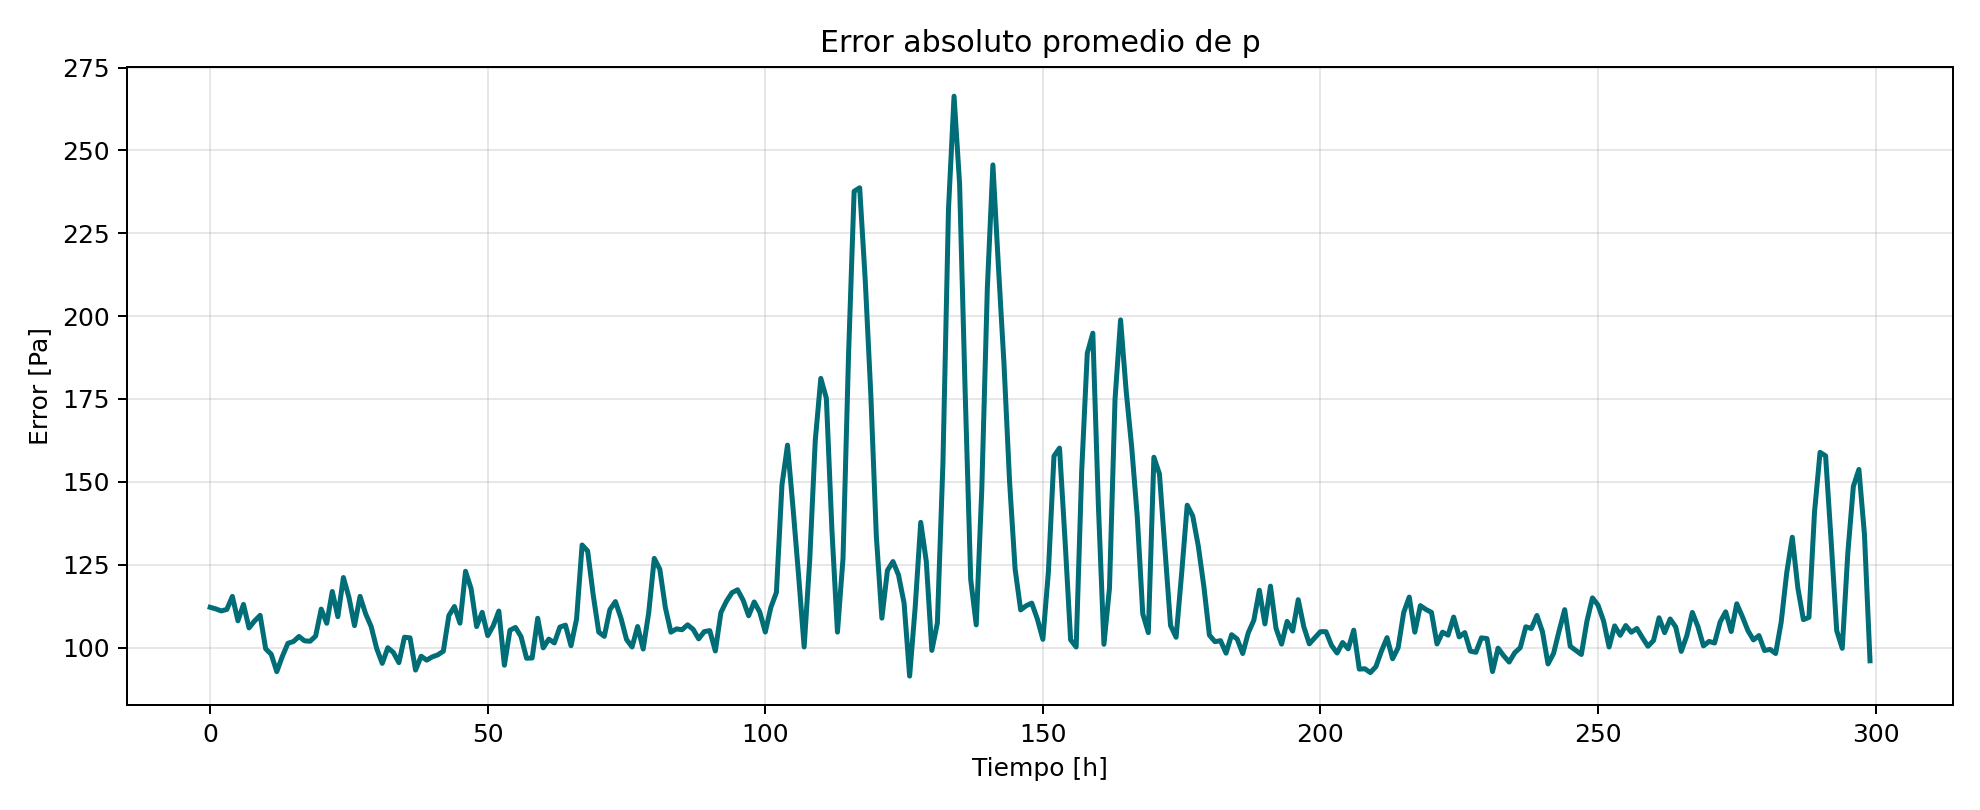
\includegraphics[width=\textwidth]{Imagenes/iter_R01/PINN_caribe_excl4_300xest_R01_L5/pinn_caribe_excl4_300xest_r01_l5_epoca_2000_error_promedio_p_tiempo.png}
  \caption{Error absoluto promedio de la presion $p$ en Pa.}
\end{subfigure}
\caption{Error absoluto promedio en funcion del tiempo para la corrida \texttt{R01\_L5} ($R=0{,}1^\circ$, $\lambda=5$), epoca 2000.}
\label{fig:error_r01_l5}
\end{figure}

\begin{figure}[H]
\centering
\begin{subfigure}[b]{0.85\textwidth}
  \centering
  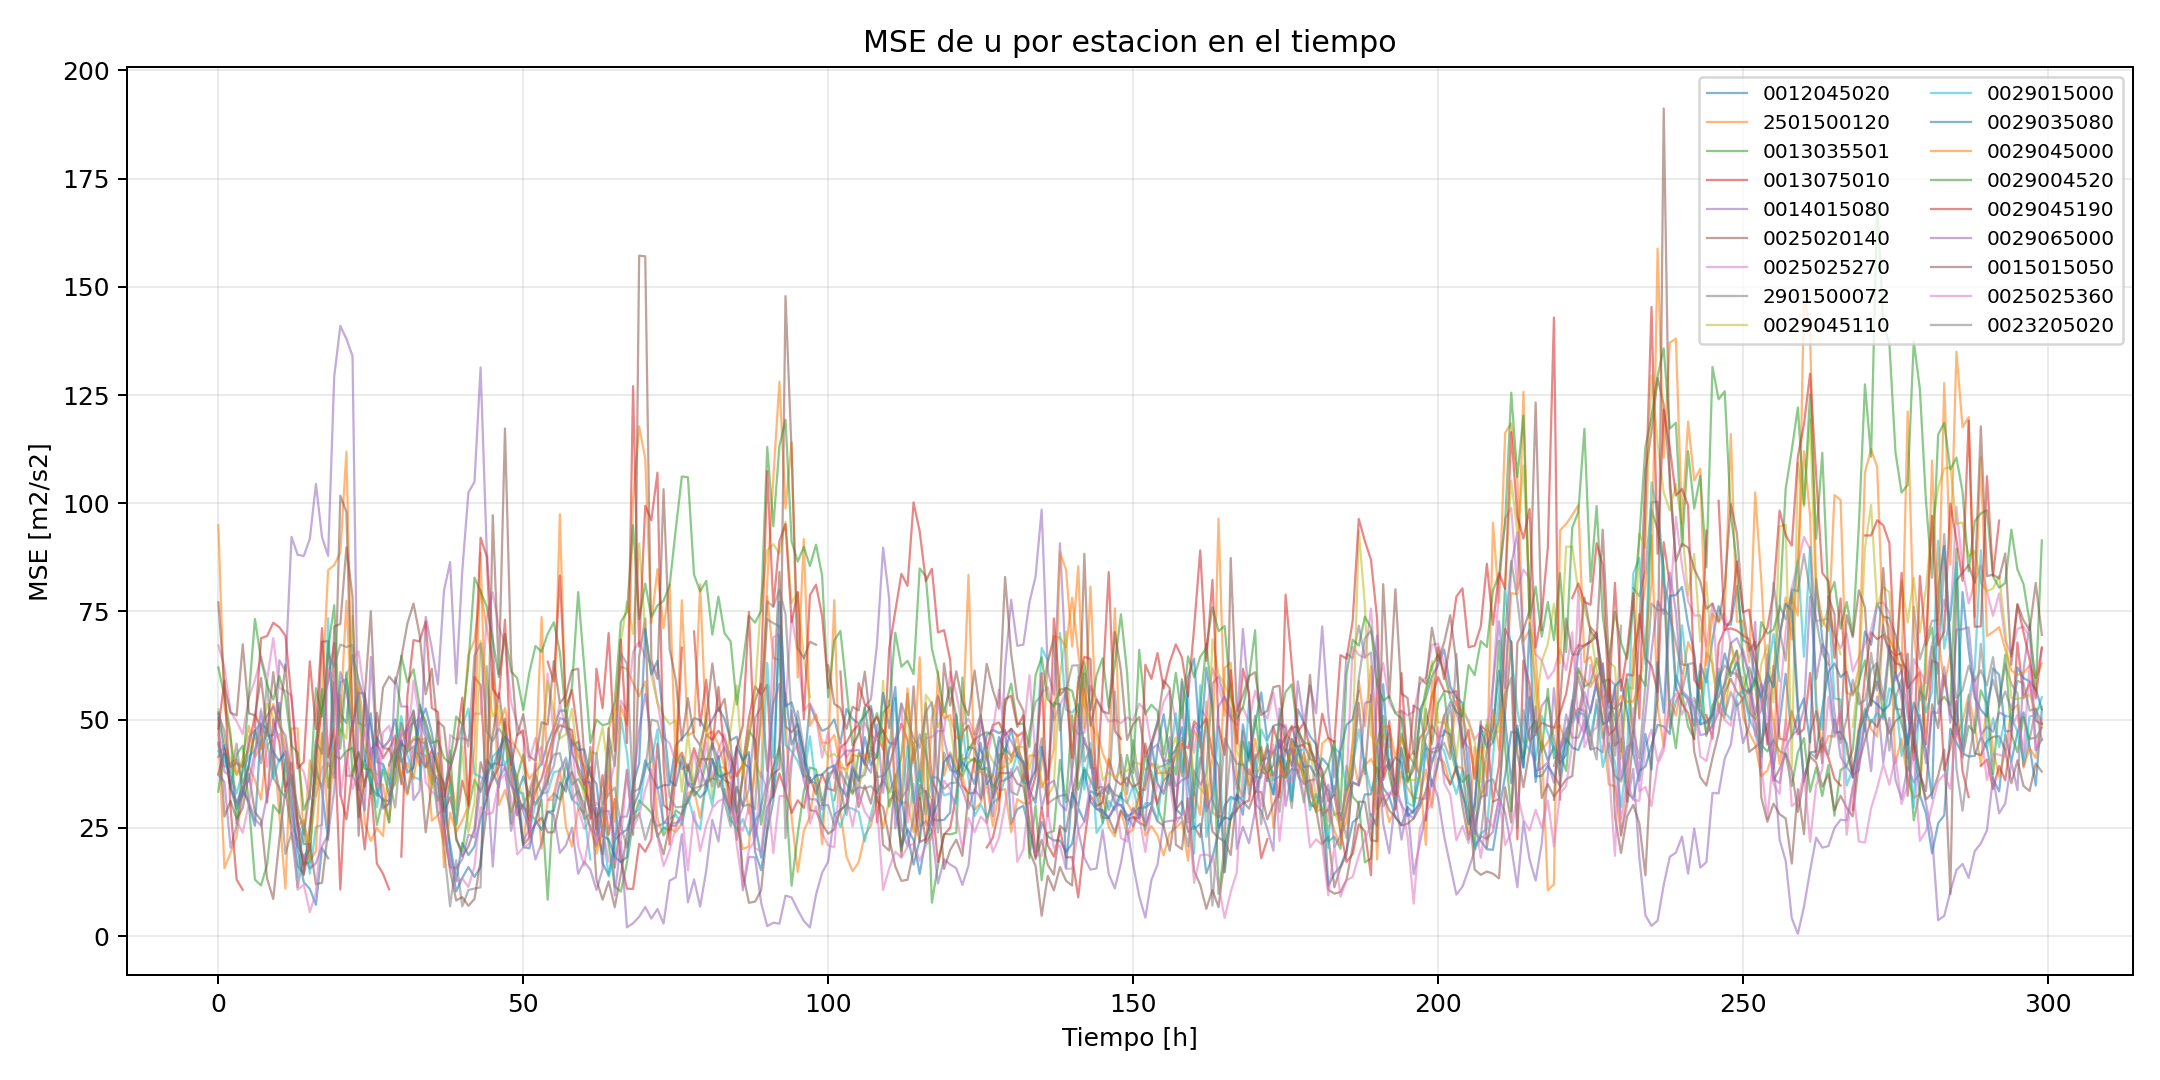
\includegraphics[width=\textwidth]{Imagenes/iter_R01/PINN_caribe_excl4_300xest_R01_L5/pinn_caribe_excl4_300xest_r01_l5_epoca_2000_mse_por_estacion_u_tiempo.png}
  \caption{MSE de la componente $u$ por estacion en m$^2$/s$^2$.}
\end{subfigure}
\par\medskip
\begin{subfigure}[b]{0.85\textwidth}
  \centering
  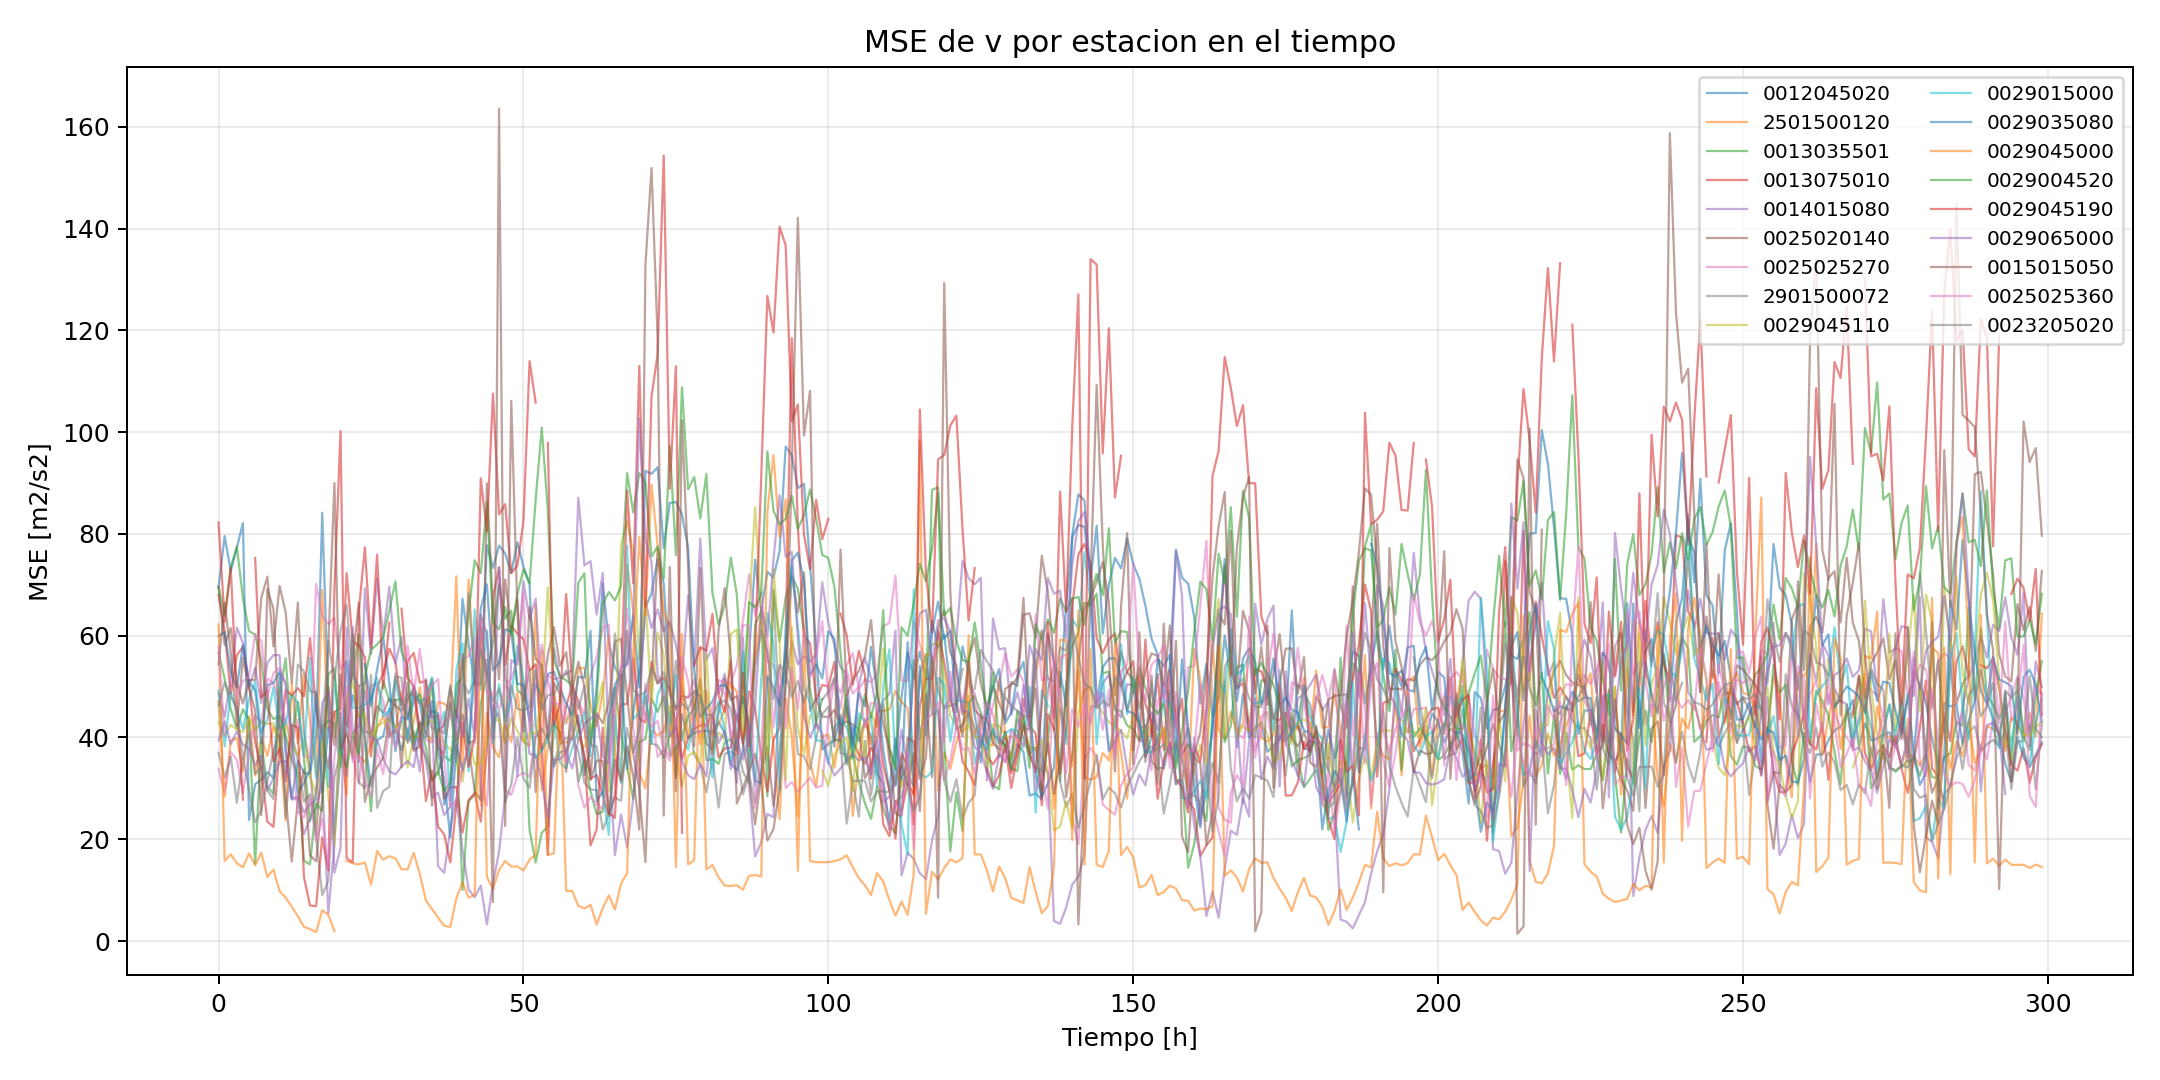
\includegraphics[width=\textwidth]{Imagenes/iter_R01/PINN_caribe_excl4_300xest_R01_L5/pinn_caribe_excl4_300xest_r01_l5_epoca_2000_mse_por_estacion_v_tiempo.png}
  \caption{MSE de la componente $v$ por estacion en m$^2$/s$^2$.}
\end{subfigure}
\par\medskip
\begin{subfigure}[b]{0.85\textwidth}
  \centering
  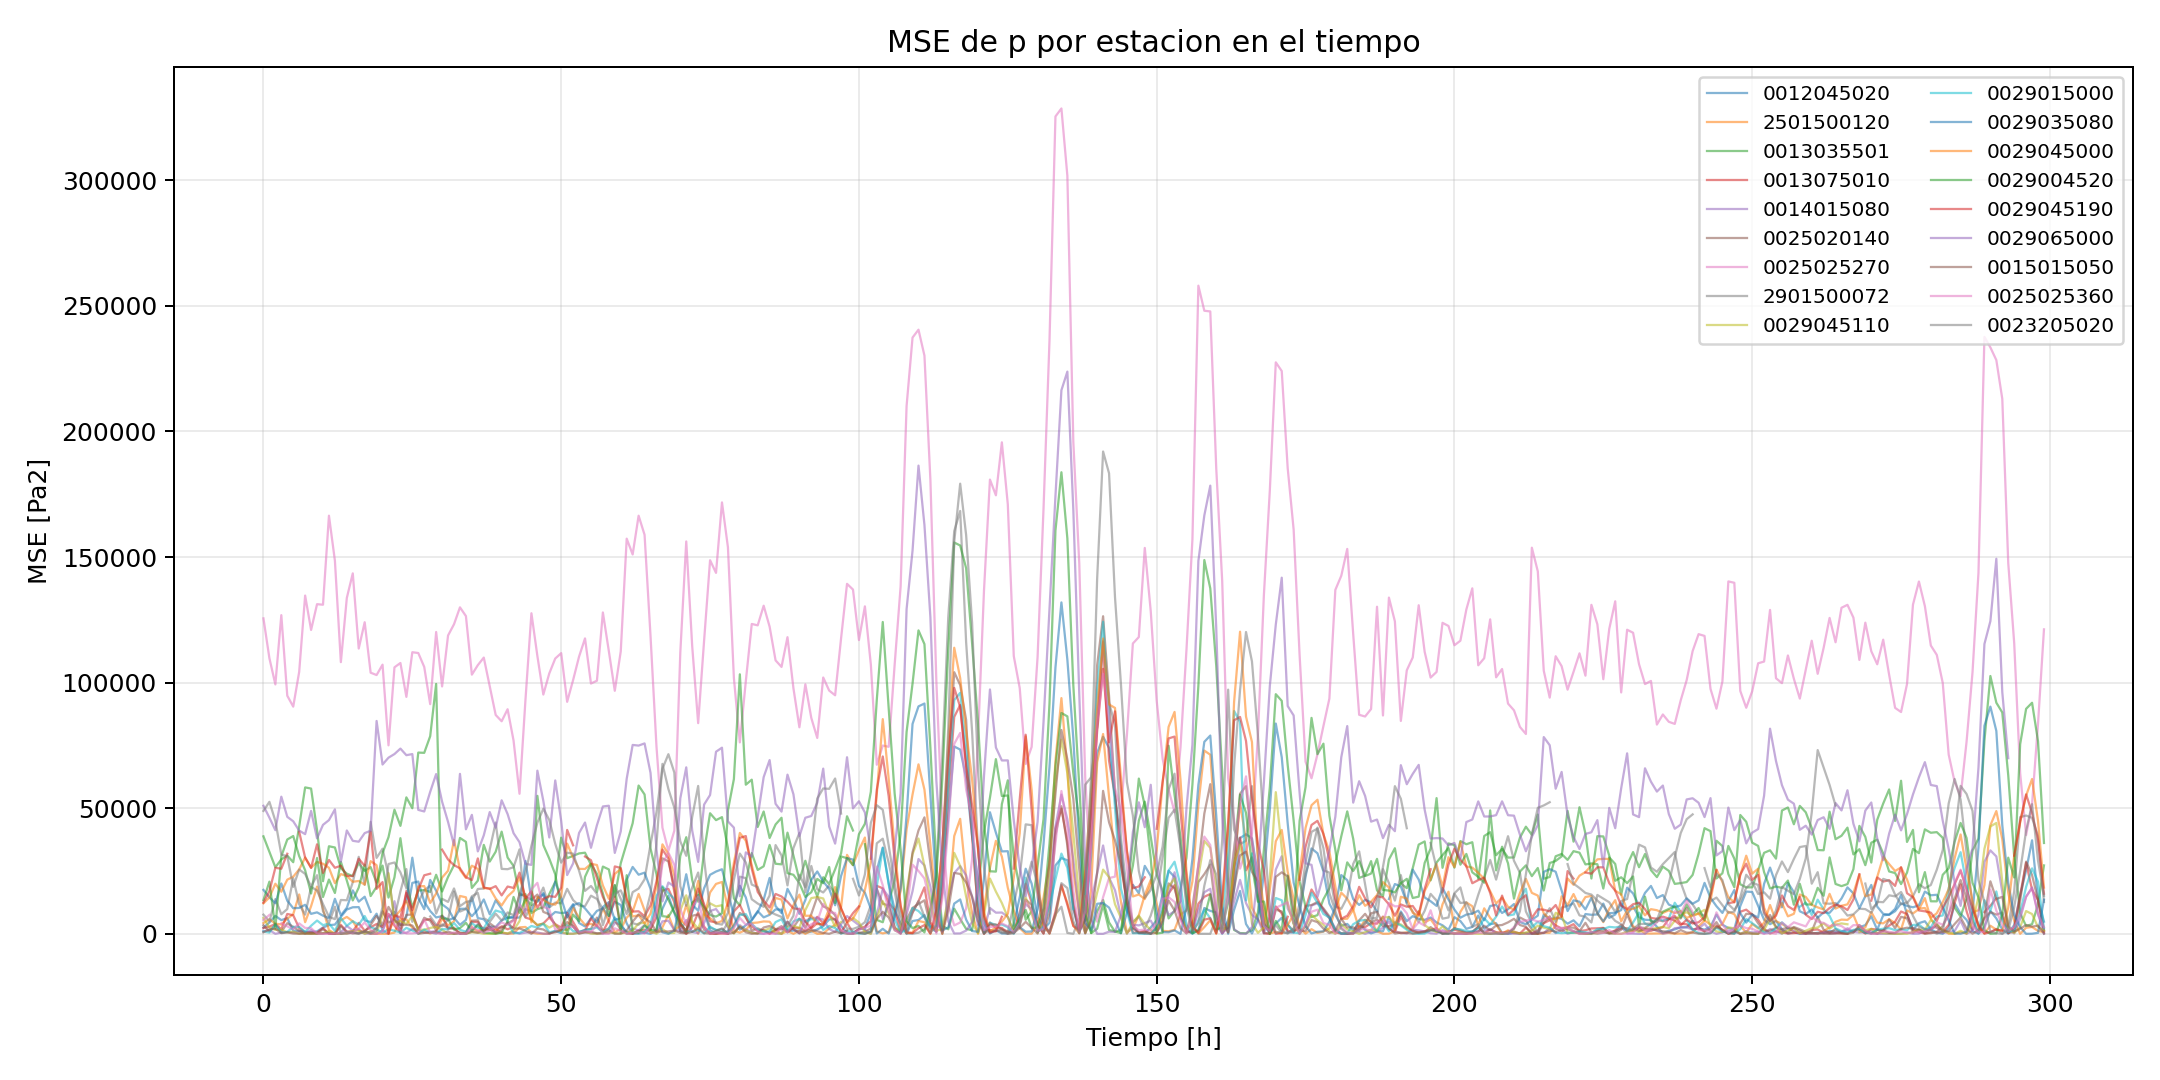
\includegraphics[width=\textwidth]{Imagenes/iter_R01/PINN_caribe_excl4_300xest_R01_L5/pinn_caribe_excl4_300xest_r01_l5_epoca_2000_mse_por_estacion_p_tiempo.png}
  \caption{MSE de la presion $p$ por estacion en Pa$^2$.}
\end{subfigure}
\caption{MSE por estacion en funcion del tiempo para la corrida \texttt{R01\_L5}, epoca 2000.}
\label{fig:mse_r01_l5}
\end{figure}

Las Figuras~\ref{fig:error_r04_l1} y~\ref{fig:mse_r04_l1} presentan la configuracion \texttt{R04\_L1}, que fue la mejor del bloque $R=0{,}4^\circ$ en criterio observacional.

\begin{figure}[H]
\centering
\begin{subfigure}[b]{0.85\textwidth}
  \centering
  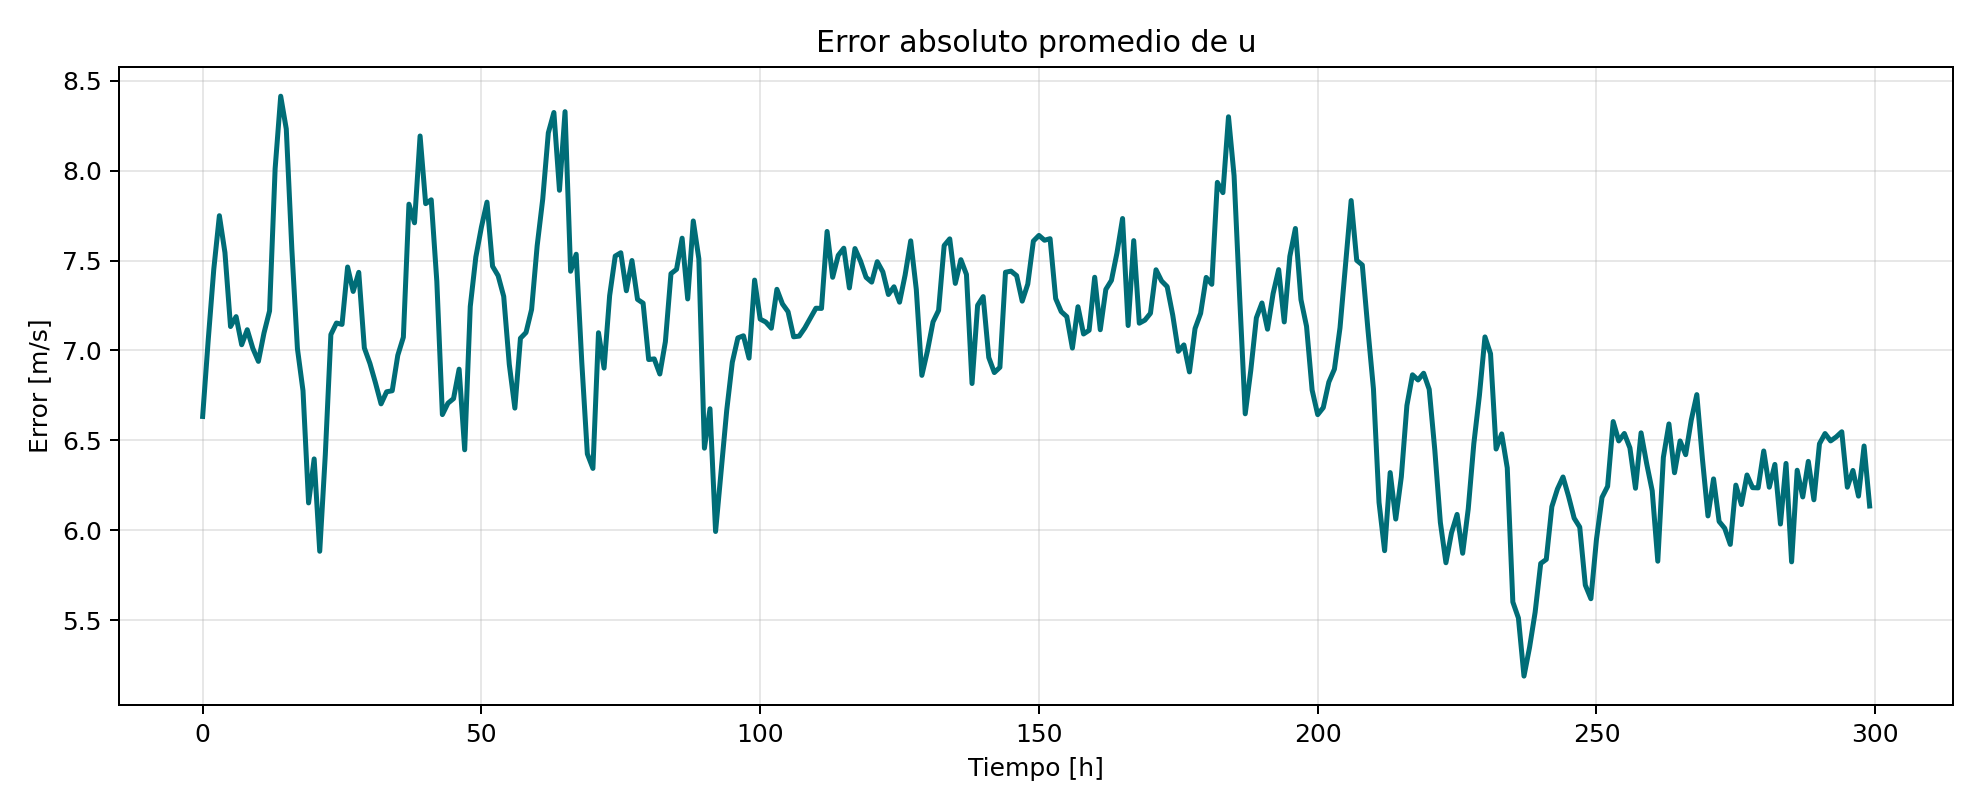
\includegraphics[width=\textwidth]{Imagenes/iter_R04_analisis_20260423/PINN_caribe_excl4_300xest_R04_L1/pinn_caribe_excl4_300xest_r04_l1_epoca_2000_error_promedio_u_tiempo.png}
  \caption{Error absoluto promedio de la componente $u$ (Este--Oeste) en m/s.}
\end{subfigure}
\par\medskip
\begin{subfigure}[b]{0.85\textwidth}
  \centering
  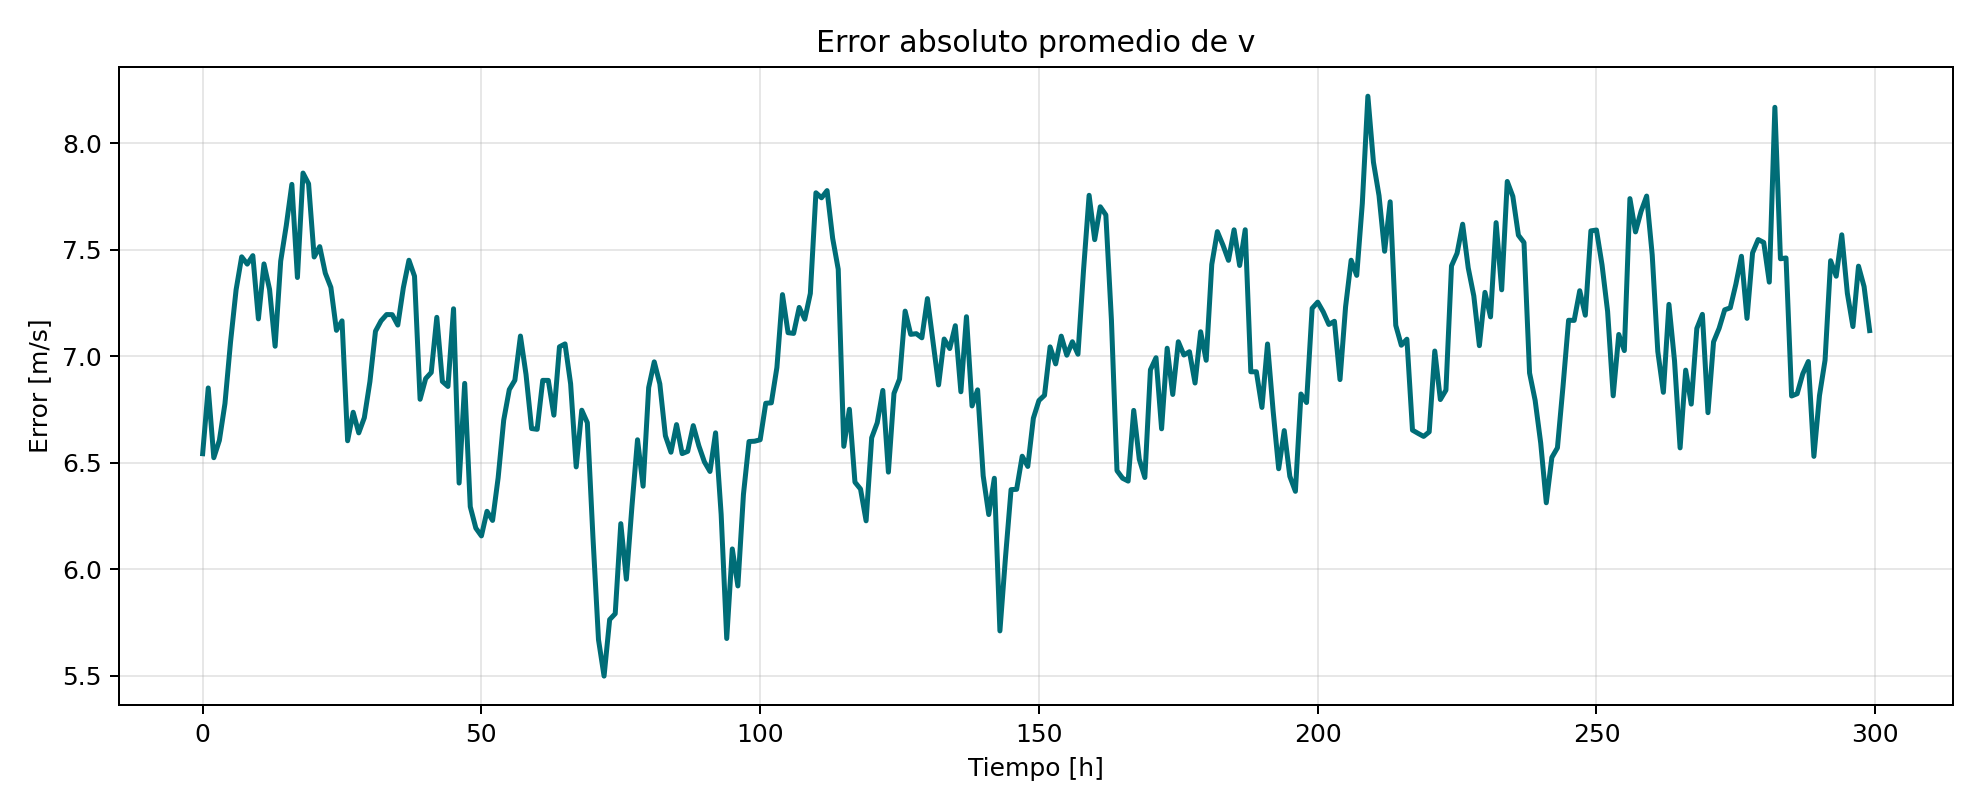
\includegraphics[width=\textwidth]{Imagenes/iter_R04_analisis_20260423/PINN_caribe_excl4_300xest_R04_L1/pinn_caribe_excl4_300xest_r04_l1_epoca_2000_error_promedio_v_tiempo.png}
  \caption{Error absoluto promedio de la componente $v$ (Norte--Sur) en m/s.}
\end{subfigure}
\par\medskip
\begin{subfigure}[b]{0.85\textwidth}
  \centering
  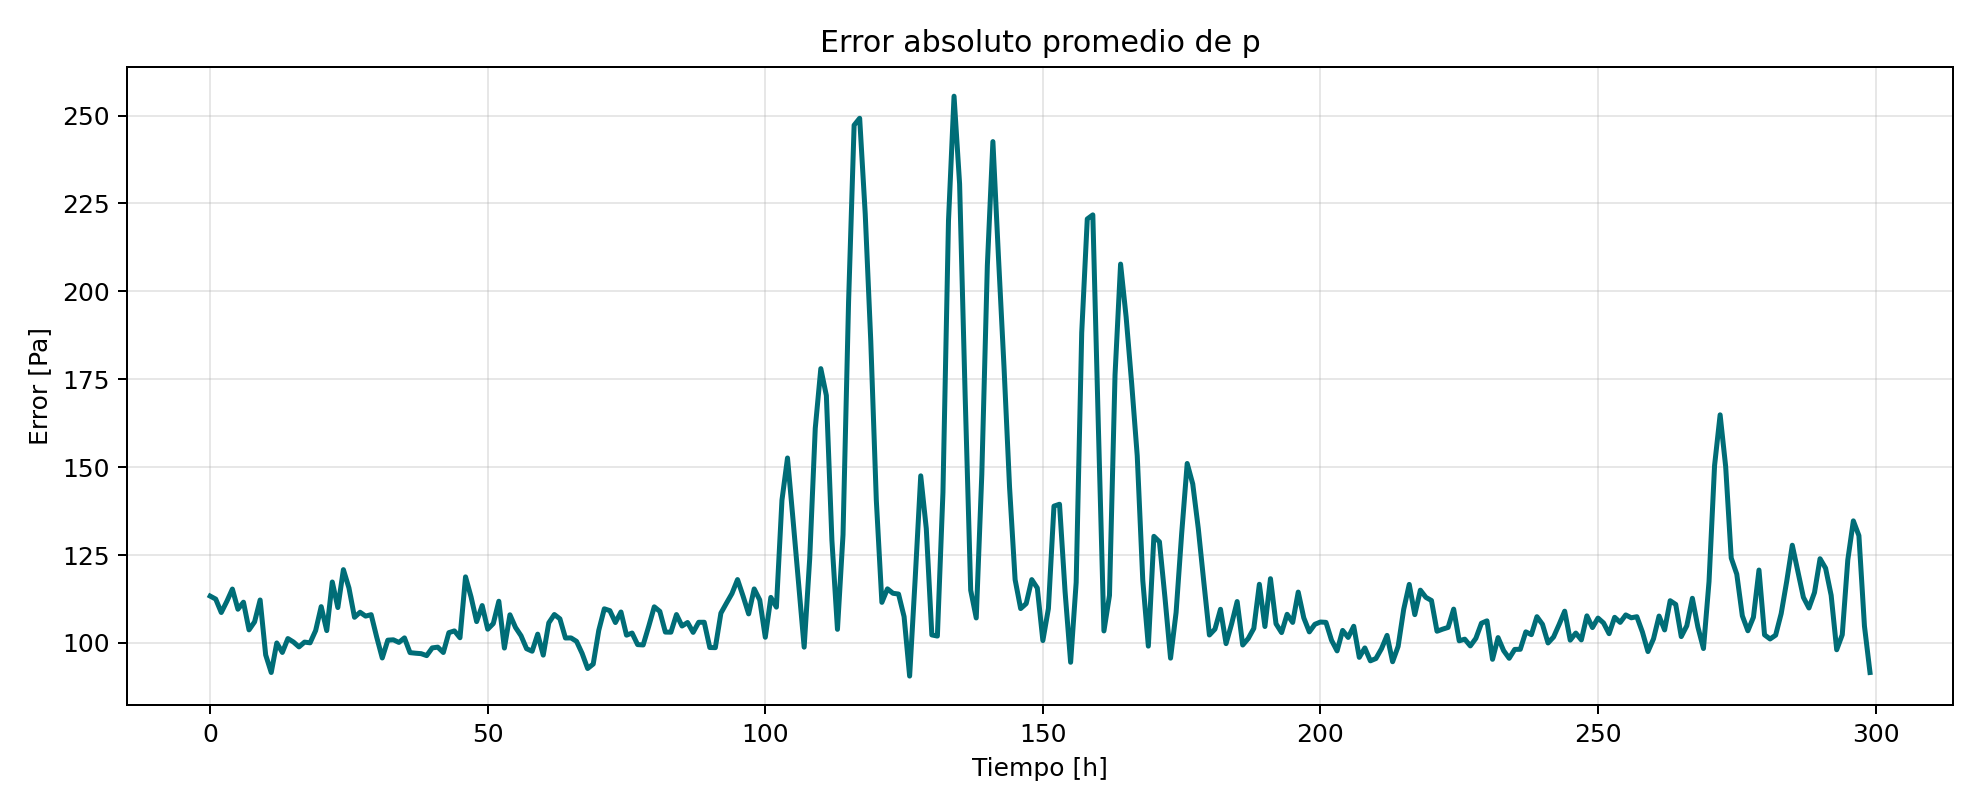
\includegraphics[width=\textwidth]{Imagenes/iter_R04_analisis_20260423/PINN_caribe_excl4_300xest_R04_L1/pinn_caribe_excl4_300xest_r04_l1_epoca_2000_error_promedio_p_tiempo.png}
  \caption{Error absoluto promedio de la presion $p$ en Pa.}
\end{subfigure}
\caption{Error absoluto promedio en funcion del tiempo para \texttt{R04\_L1} ($R=0{,}4^\circ$, $\lambda=1$), epoca 2000.}
\label{fig:error_r04_l1}
\end{figure}

\begin{figure}[H]
\centering
\begin{subfigure}[b]{0.85\textwidth}
  \centering
  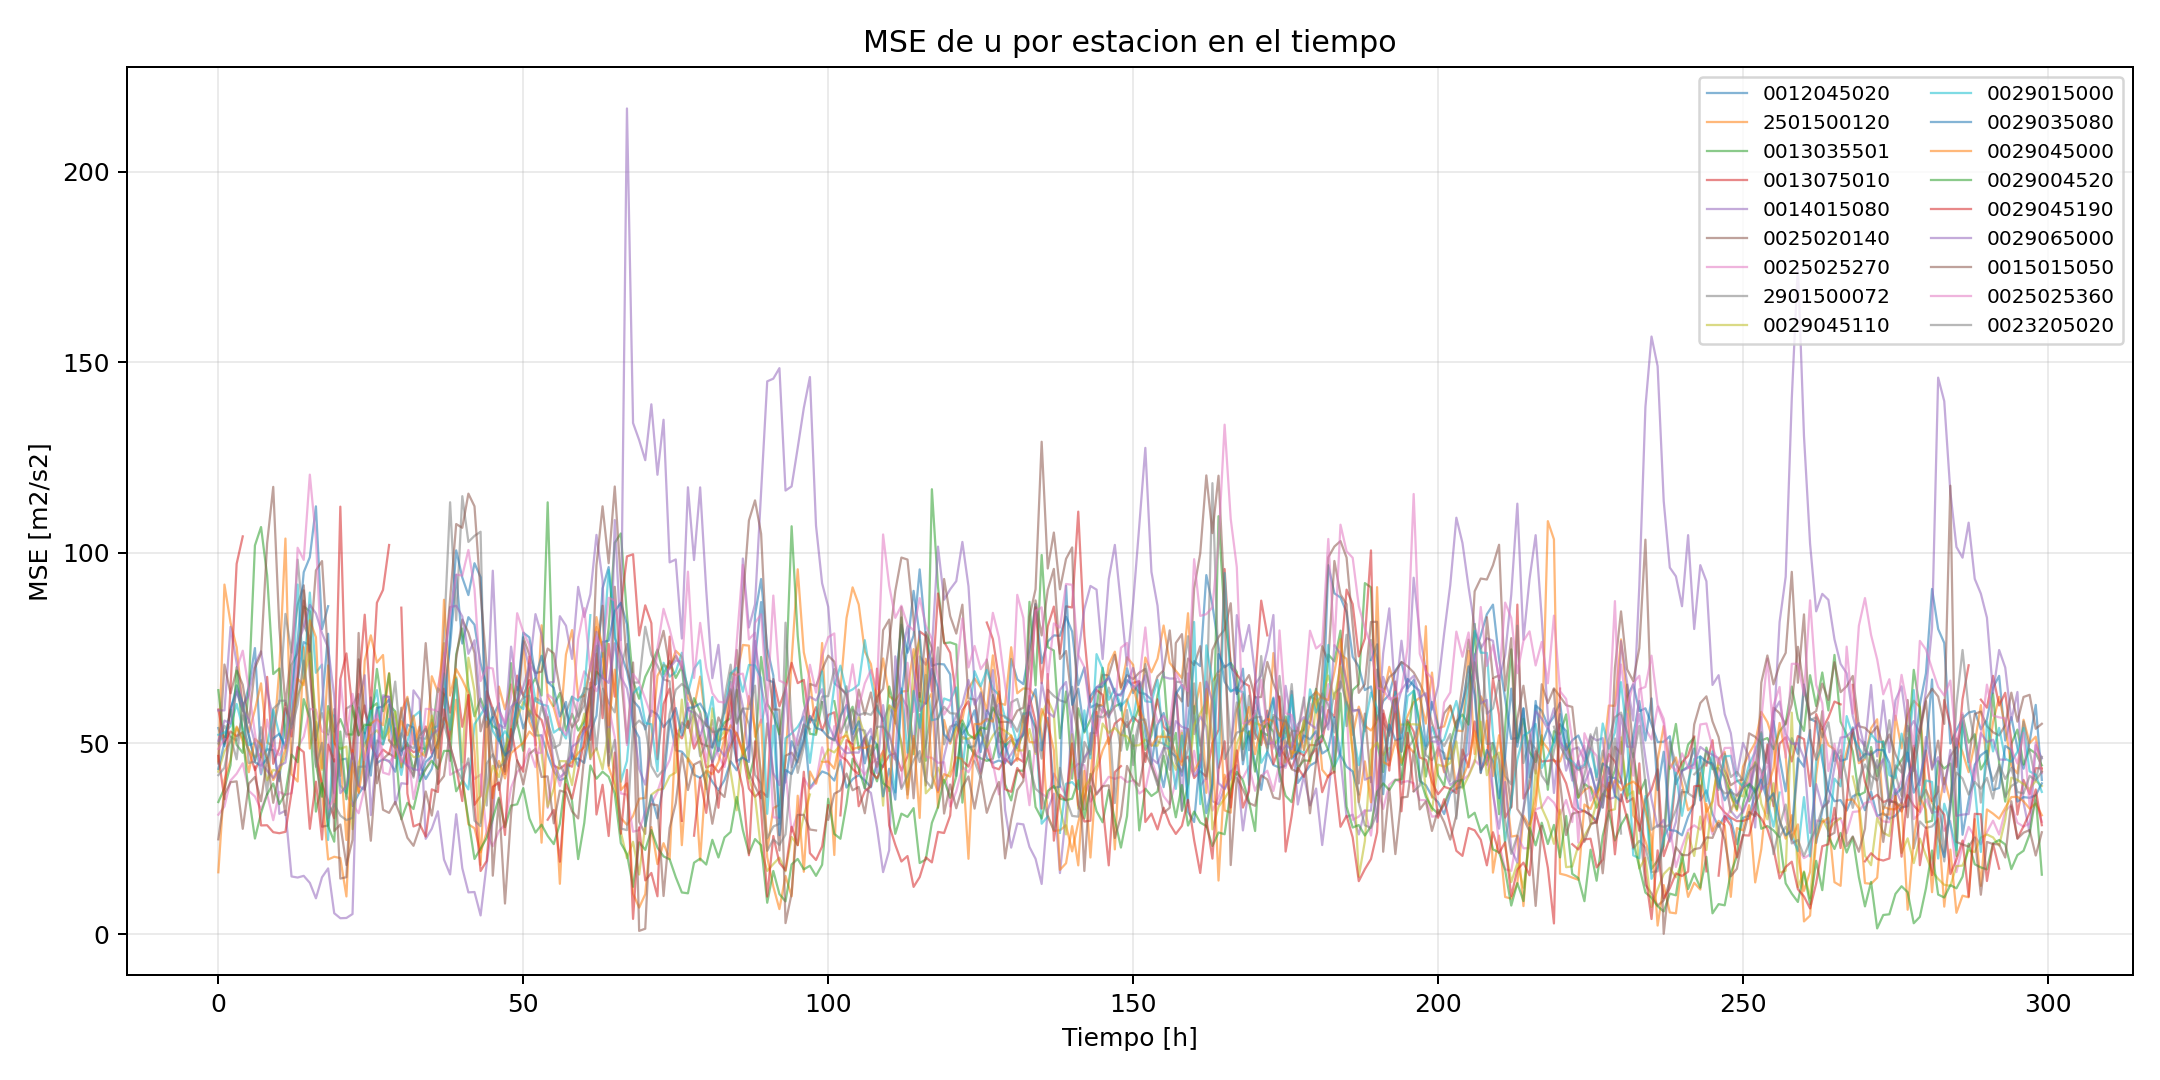
\includegraphics[width=\textwidth]{Imagenes/iter_R04_analisis_20260423/PINN_caribe_excl4_300xest_R04_L1/pinn_caribe_excl4_300xest_r04_l1_epoca_2000_mse_por_estacion_u_tiempo.png}
  \caption{MSE de la componente $u$ por estacion en m$^2$/s$^2$.}
\end{subfigure}
\par\medskip
\begin{subfigure}[b]{0.85\textwidth}
  \centering
  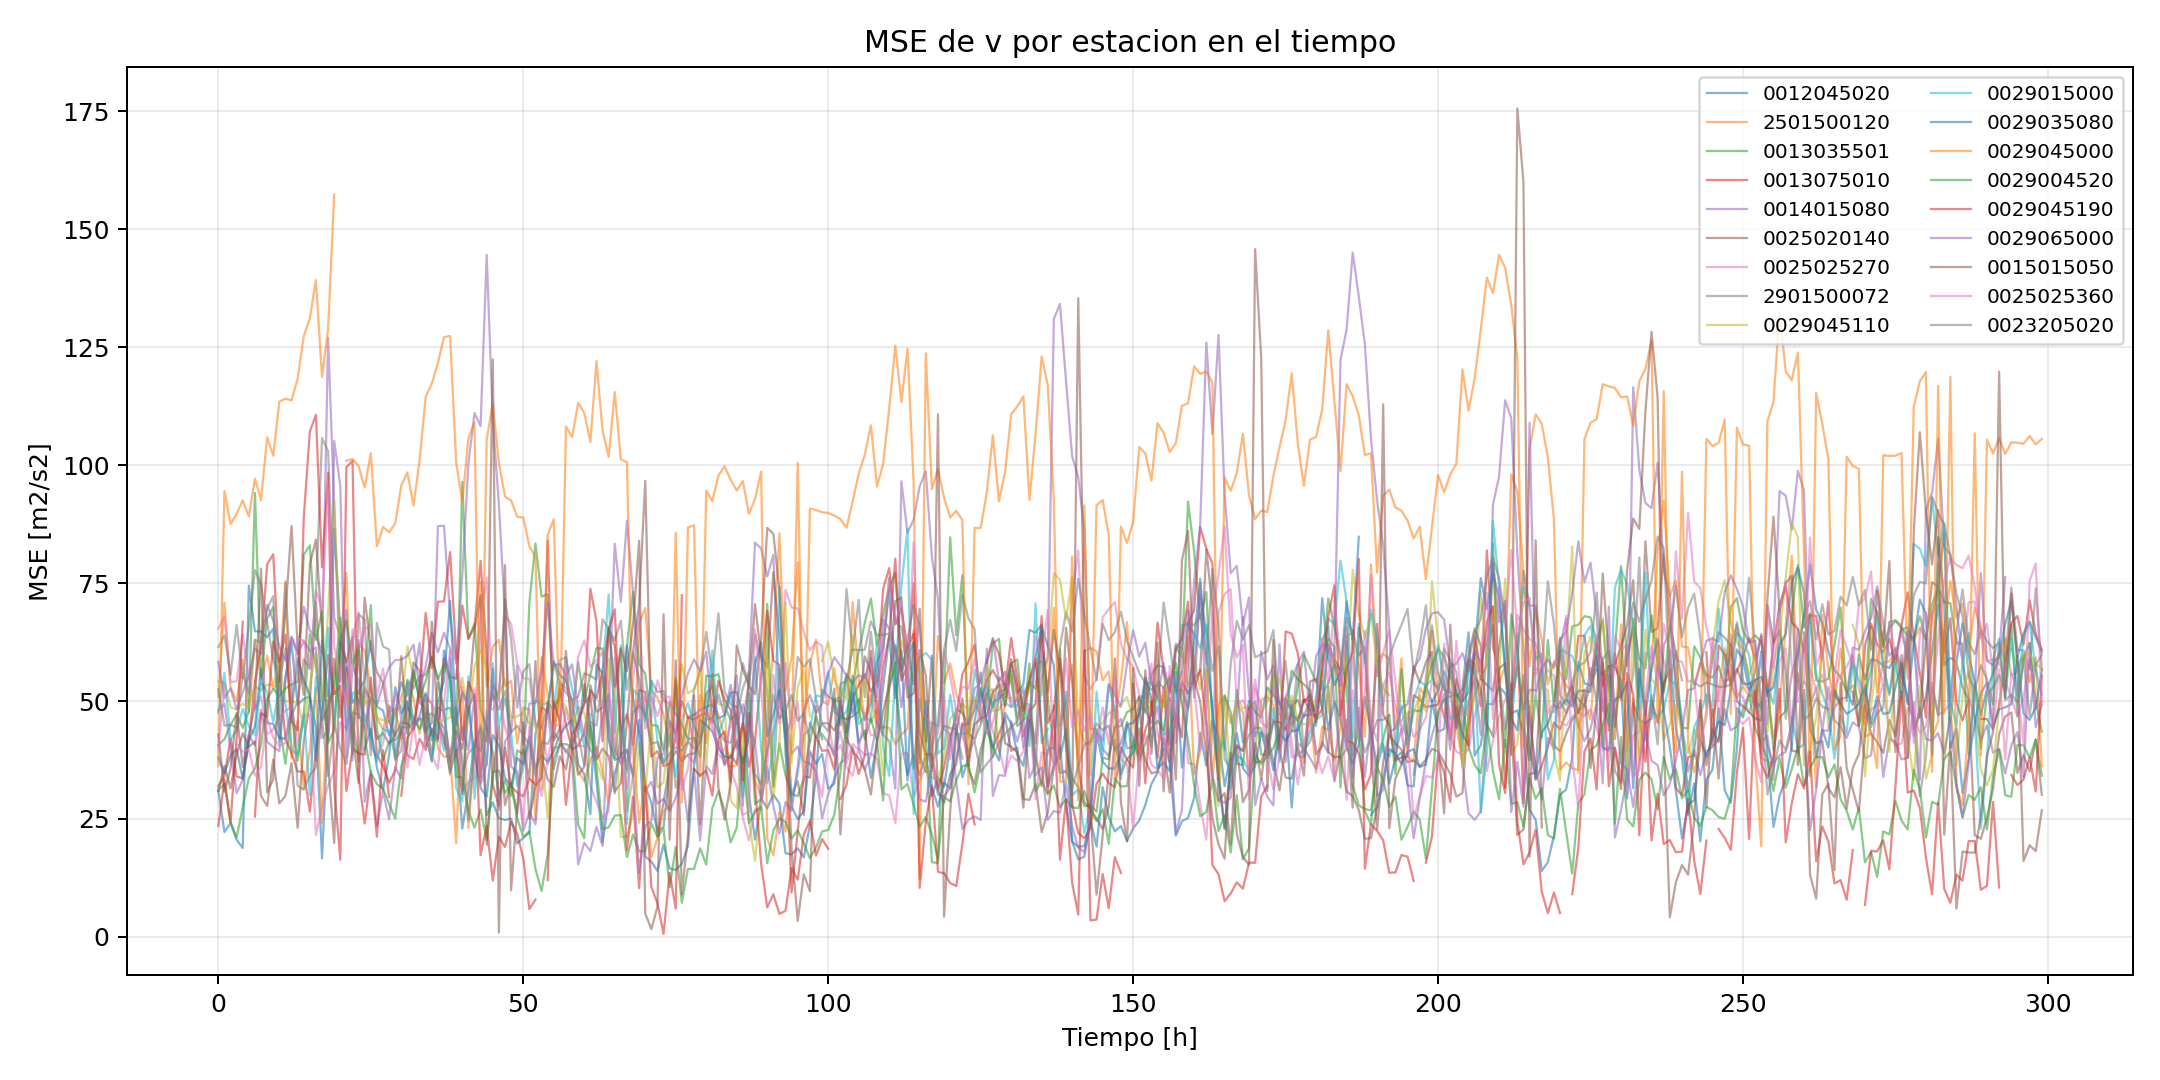
\includegraphics[width=\textwidth]{Imagenes/iter_R04_analisis_20260423/PINN_caribe_excl4_300xest_R04_L1/pinn_caribe_excl4_300xest_r04_l1_epoca_2000_mse_por_estacion_v_tiempo.png}
  \caption{MSE de la componente $v$ por estacion en m$^2$/s$^2$.}
\end{subfigure}
\par\medskip
\begin{subfigure}[b]{0.85\textwidth}
  \centering
  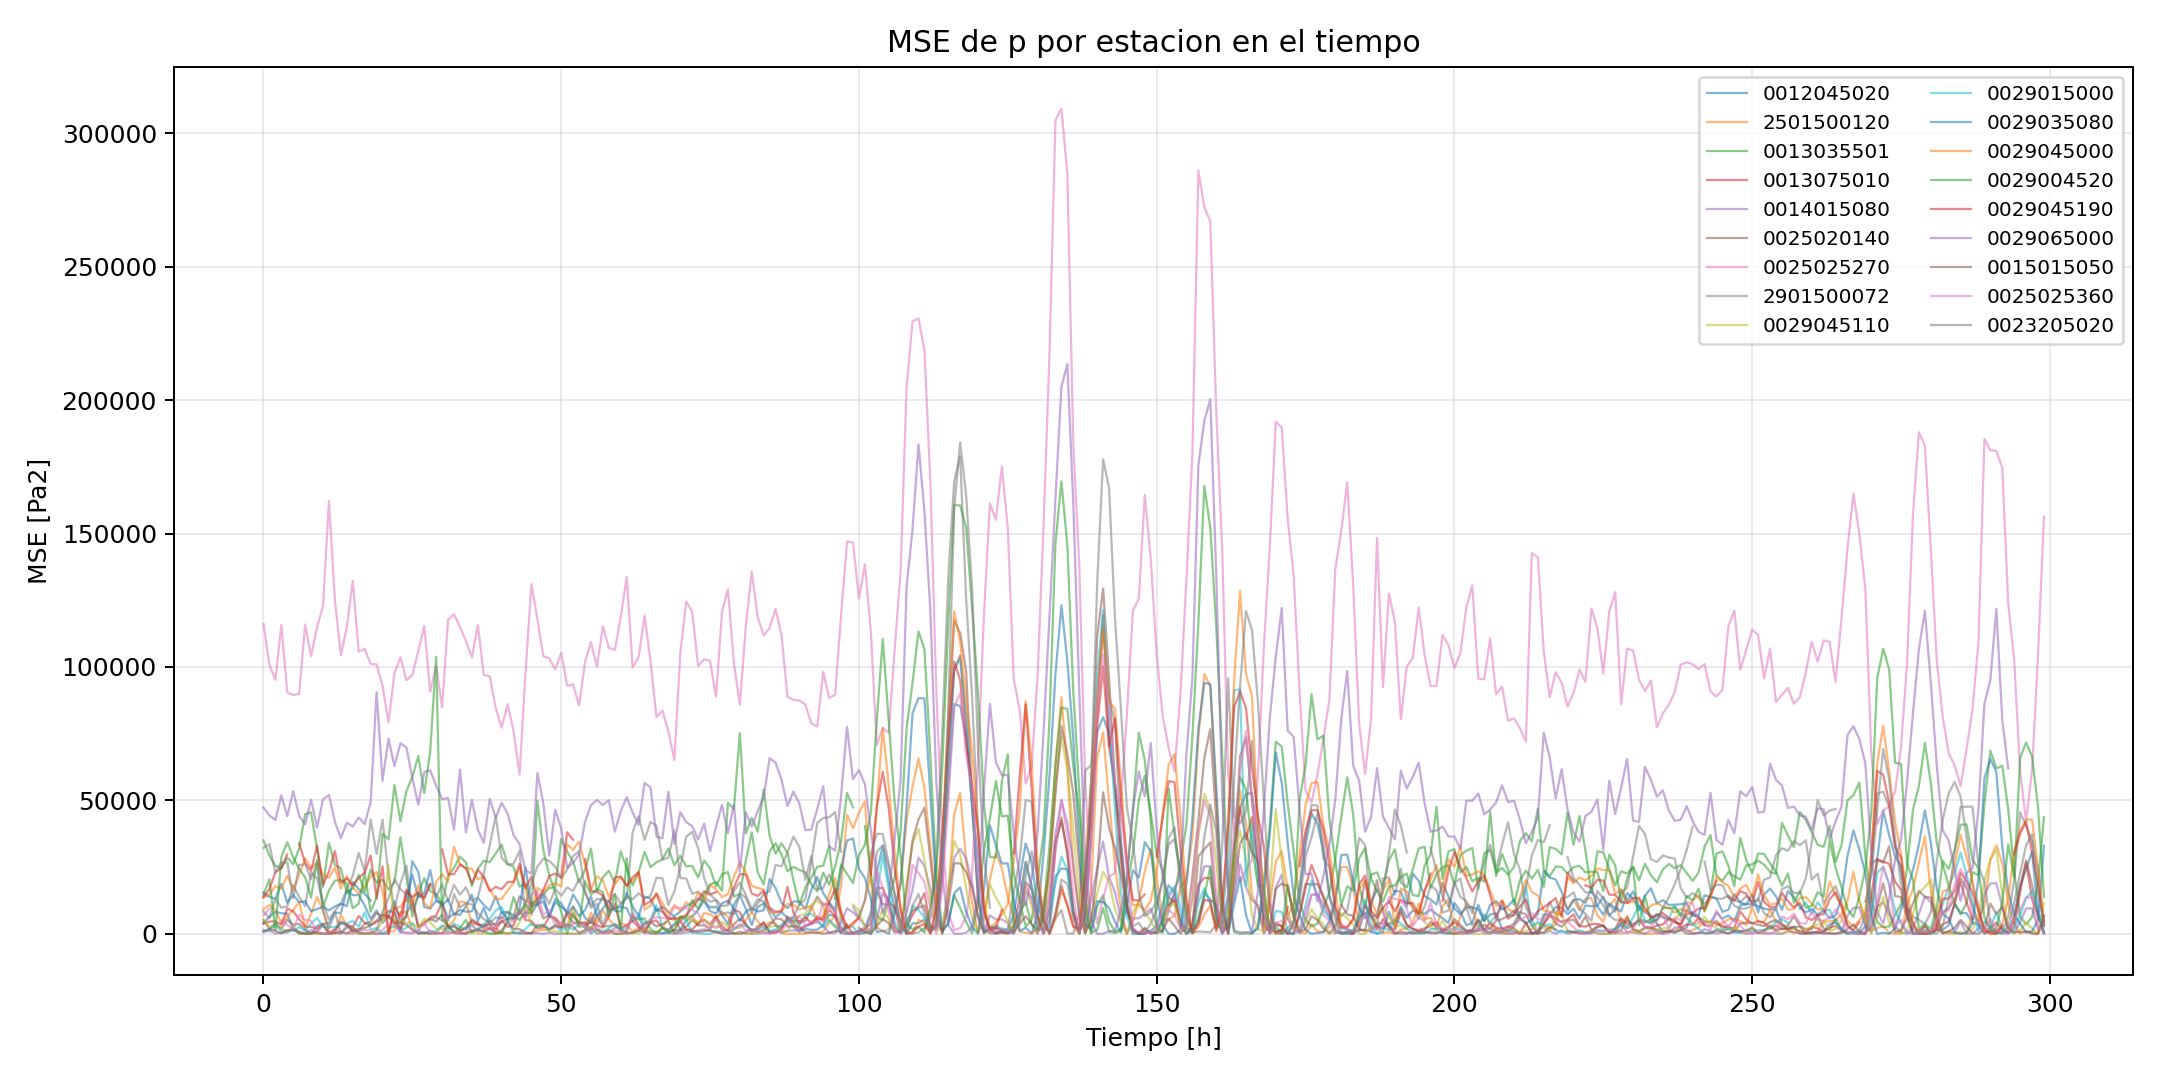
\includegraphics[width=\textwidth]{Imagenes/iter_R04_analisis_20260423/PINN_caribe_excl4_300xest_R04_L1/pinn_caribe_excl4_300xest_r04_l1_epoca_2000_mse_por_estacion_p_tiempo.png}
  \caption{MSE de la presion $p$ por estacion en Pa$^2$.}
\end{subfigure}
\caption{MSE por estacion en funcion del tiempo para \texttt{R04\_L1}, epoca 2000.}
\label{fig:mse_r04_l1}
\end{figure}
